\chapter{Must-Link Constraints for Video Segmentation}
\label{Chapter5}
In this chapter we propose a methodology for discriminative learning of must-link constraints and their incorporation in the video segmentation framework.

First we introduce a way of integrating prior information in the form of must-link constraints into spectral clustering while preserving all the
balanced graph cuts, which was presented in the work of~\cite{RangapuramH12}.
Then we continue with the analysis of low-level features as must-link constraints and graph connectivity in order to explore how much the performance can be boosted based on the connections in the graph.

Further we suggest to learn must-links with Random Forests classifier from low-level features.
Then we compare the performance of spectral clustering and 1-spectral clustering in the proposed constrained setting.  
We show that even a naive learning approach on the restricted feature space can improve segmentation results. 
As a final step the proposed method is compared with existing state-of-the-art algorithms.
%These experiments showed us that employing constrained spectral clustering can significantly improve the performance and reduce the runtime of the algorithm.
%Further the generalization of 1-spectral clustering which integrates must-link constraints, the method called COSC~\cite{RangapuramH12}, is presented. 
\section{Integration of Must-Link Constraints into Video Segmentation}
\label{sec:ch5_cosc}
In the recent work~\cite{Galasso14} employing the constrained spectral clustering has shown to be beneficial for video segmentation, as it not only uses some prior knowledge and therefore constrains the solution, 
but also reduces the graph and the complexity of the algorithm. 
% The method is called COSC and is based on an optimization technique RatioDCA proposed in~\cite{HeinS11}.
% In the similar spirit as for 1-spectral clustering, they show a tight relaxation of the constrained normalized cut problem into an unconstrained continuous optimization problem.
% While the convergence to the global optimum is not guaranteed,
Both the graph reduction and integration of must-link constraints have been addressed by the work of~\cite{RangapuramH12}, which suggests the generalization of spectral relaxations 
to the constrained setting. 

In this approach the constraints are enforced by direct manipulation of the graph, then unconstrained spectral clustering can be applied
on the new reduced graph. If the must-link constraints are reliable they can be directly integrated by merging the corresponding vertices of the graph together and redefining the edge and vertex weights. This way of constructing 
the reduced graph preserves all normalized cuts which respect the must-link constraints and improves the partition compared to the unconstrained case (see fig.~\ref{fig:cosc}).
\begin{figure}[htbp]
\centering
\subfigure[A simple graph in two dimensions]{%
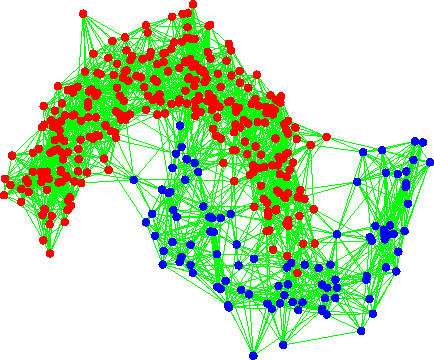
\includegraphics[width=0.23\textwidth]{images/png/cosc_1.png}
\label{fig:subfigure1}}
\subfigure[Must-link constraints]{%
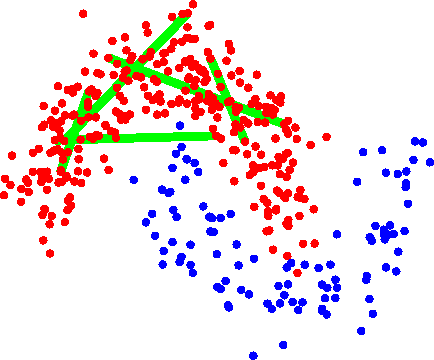
\includegraphics[width=0.23\textwidth]{images/png/cosc_2.png}
\label{fig:subfigure2}}
\subfigure[Unconstrained clustering]{%
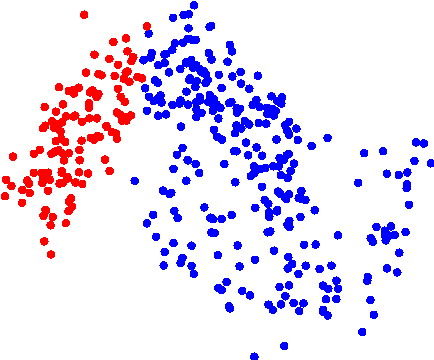
\includegraphics[width=0.23\textwidth]{images/png/cosc_3.png}
\label{fig:subfigure1}}
\subfigure[Constrained clustering]{%
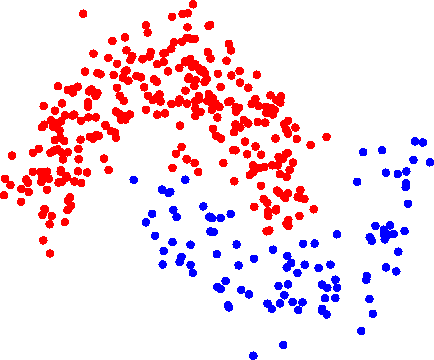
\includegraphics[width=0.23\textwidth]{images/png/cosc_4.png}
\label{fig:subfigure2}}
\caption[Clustering without constraints vs. constrained clustering]{
 {\bf Clustering without constraints vs. constrained clustering} (courtesy of~\cite{Hein13}).}
\label{fig:cosc}
\end{figure}

%The must-link constraint indicate that the two objects should lie in the same cluster. 
The scheme for the construction of a reduced graph for a must-link constraint $(p,q)$ is given below:
\begin{enumerate}
 \item merge $p$ and $q$ into a single vertex $\tau$;
\item update the vertex weight of $\tau$ by $b_{\tau} = b_p+b_q$;
\item update the edges as follows: if $r$ is any vertex other than $p$ and $q$, then add an edge between $\tau$ and $r$ with weight $w(p,r)+w(q,r)$.
\end{enumerate}

Using this scheme one can efficiently integrate many must-links together, by first constructing the must-link constraint graph and merging each connected component in this way. Note that even if the original graph
has vertex weights equal to one this construction leads to a graph with vertex weights.

All partitions of the reduced graph fulfill the must-link constraints and hence any relaxation of the unconstrained cut problem can now be applied. This is not restricted to the particular balanced graph cut criterion as long as
the cut and the volume of the subsets are preserved in the reduction. 

In this thesis we would like to adopt this approach to the setting where the additional information in the form of must-link constraints is learned from 
the low-level features of the video and then integrated into segmentation framework, presented in Section~\ref{sec:ch3_framework}.

The outline of the proposed model is listed in Algorithm~\ref{alg:VSM_ML}. 
\incmargin{1em} 
\begin{algorithm}[htbp]
\caption{Proposed Video Segmentation Model with Must-Link Constraints}
\label{alg:VSM_ML}
\DontPrintSemicolon
\BlankLine
\Indm  
\Setnlsty{textbf}{}{:}
\Indp
\BlankLine
extract superpixels from the lowest hierarchical level of pixel-based segmentation, obtained via MAHIS;\\
compute low-level video features based on superpixels;\\ 
construct a graph with an affinity matrix formed of pair-wise within- and between-frame similarity measures;\\
learn with Random Forests must-link constraints from low-level features;\\
construct the reduced graph by integrating must-link constraints via sparsification;\\
apply spectral clustering technique for partitioning of the new reduced graph to obtain final video segmentation.
\BlankLine
\Indm  
\end{algorithm}
\decmargin{1em}
\section{Low-Level Features and Must-link Constraints}
\label{sec:llf}
%\subsection{Affinities as Must-Link Constraints}
From the described in Section~\ref{sec:ch3_aff} experiments the good performance of the low-level features was observed. Therefore integrating affinities as a side knowledge in the form of must-link constraints 
into spectral clustering could have a positive influence on the overall performance of the algorithm.
Thus we conducted the experiments, where we employed 3 best cases as the constraints: $\mathrm{ltt\geq 0.9}$, $\mathrm{(sta=1)\cup(stm=1)}$ and $\mathrm{aba\geq 0.9}$, using the most contributory to the performance features. 
As the affinities were only evaluated on the ground truth frames, the behaviour within and across other frames is still unknown and more mistakes can occur. 
For this reason we included in the experiments the oracle cases, where as must-links only connections which are known to be true based on the ground truth are used.

Figure~\ref{fig:aff_ML} illustrates boundary and volume precision-recall curves on the BMDS for the suggested settings. In these experiments we integrated must-link constraints into the standard spectral clustering framework as 
was suggested in the Section~\ref{sec:ch5_cosc}. It can be observed that on the whole employing affinities as must-links increases the performance. However, for the LTT and ABA cases, which allow a few errors, 
there is a loss in the performance in comparison with corresponding oracle cases.
Another drawback is that the number of must-link decisions that we made is quite small and does not allow to achieve a significant boost of the results.    
\begin{figure}[htbp]
\begin{minipage}[t]{1\textwidth}
 \centering
\hfill \hfill \hfill
\footnotesize $\mathrm{LTT\geq 0.9}$
\hfill \hfill \hfill
\footnotesize $\mathrm{(STA=1)\cup(STM=1)}$
\hfill \hfill \hfill
\footnotesize $\mathrm{ABA\geq 0.9}$
\hfill  \hfill \hfill 
\end{minipage}
\begin{minipage}[t]{1\textwidth}
\centering
\hfill \hfill    
\subfigure{%
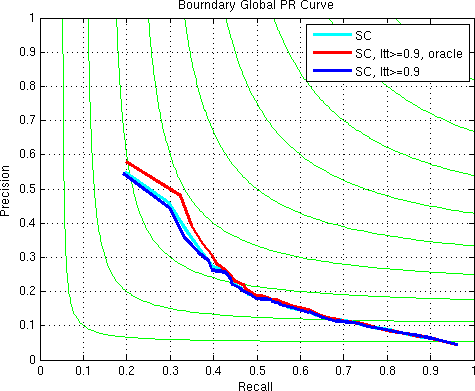
\includegraphics[trim=0cm 0cm 0cm 0.5cm, clip=true, width=0.3\textwidth]{images/aff_ml/ltt2.png}} 
\hfill  
\subfigure{%
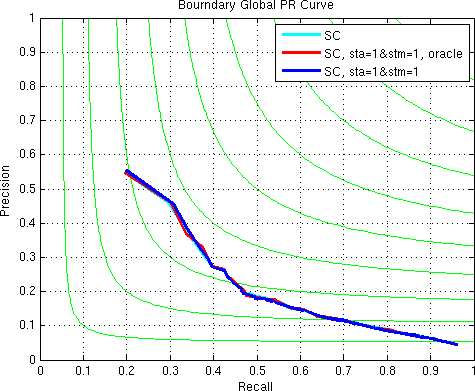
\includegraphics[trim=0cm 0cm 0cm 0.5cm, clip=true, width=0.3\textwidth]{images/aff_ml/sta2.png}} 
\hfill 
\subfigure{%
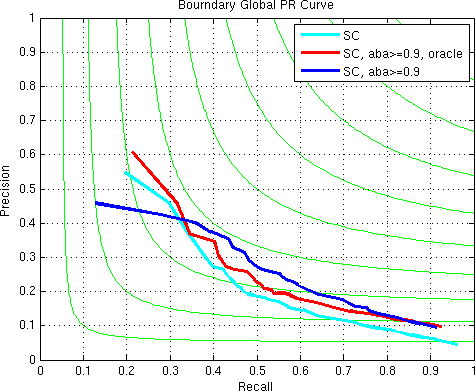
\includegraphics[trim=0cm 0cm 0cm 0.5cm, clip=true, width=0.3\textwidth]{images/aff_ml/aba2.png}} 
\hfill   \hfill

\footnotesize (a) BPR
\end{minipage}

\begin{minipage}[t]{1\textwidth}
\centering
\hfill \hfill   
\subfigure{%
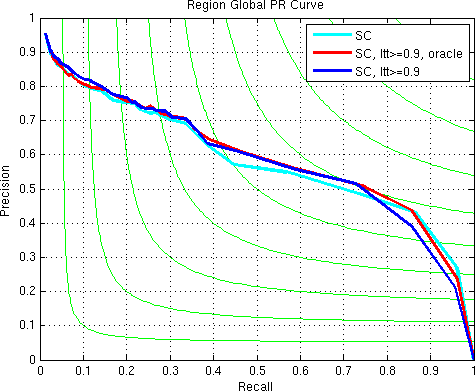
\includegraphics[trim=0cm 0cm 0cm 0.5cm, clip=true, width=0.3\textwidth]{images/aff_ml/ltt4.png}} 
\hfill  
\subfigure{%
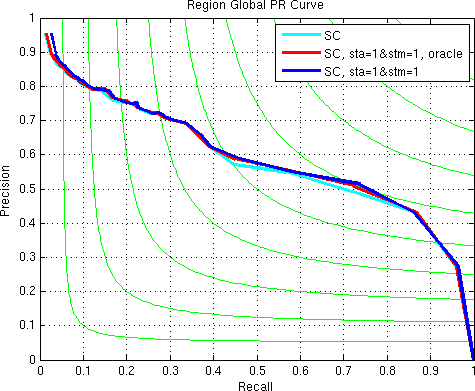
\includegraphics[trim=0cm 0cm 0cm 0.5cm, clip=true, width=0.3\textwidth]{images/aff_ml/sta4.png}} 
\hfill 
\subfigure{%
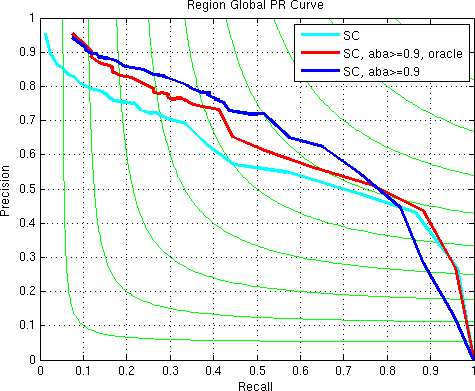
\includegraphics[trim=0cm 0cm 0cm 0.5cm, clip=true, width=0.3\textwidth]{images/aff_ml/aba4.png}} 
\hfill   \hfill

\footnotesize (b) VPR
\end{minipage}

\caption[Boundary precision-recall (BPR) and volume precision-recall (VPR) curves for spectral clustering (SC) using thresholded affinity measures as must-links]{
{\bf Boundary precision-recall (BPR) and volume precision-recall (VPR) curves for spectral clustering (SC) using thresholded affinity measures as must-links.} We consider 3 cases as must-link constraints:
$\mathrm{ltt\geq 0.9}$, $\mathrm{(sta=1)\cup(stm=1)}$, $\mathrm{aba\geq 0.9}$, where the red curves represent the oracle.}
\label{fig:aff_ML}
\end{figure}

%\subsection{Exploring Connections in the Graph }
It has been shown above that the prior information can be gained from low-level features and the performance of video segmentation can be increased by integrating must-links constraints.
In the next experiment the goal was to explore how much the performance can be boosted by employing must-links.
For this purpose we considered all the true connections in the graph as must-link constraints. All the connected in the graph superpixels which belong to the same object according to the ground truth were merged together.
We distinguished 3 types of connections: within-frame, between-frame and a combination of both. For each case 100\% and 1\% of all possible merges were considered. It is worth saying
that all must-link decisions were restricted to the annotated frames of the video sequence.

The results of the experiment are presented in Figure~\ref{fig:aff_conn}. One can observe that the connectivity of the graph allows a significant improvement of the performance, even if a single type of connections is considered. 
Just by merging within-frame much better segmentations can be achieved. The only condition is that the number of must-link constraints must be big enough to have an impact on the final performance. 
\begin{figure}[htbp]
 \centering
\subfigure[BPR]{%
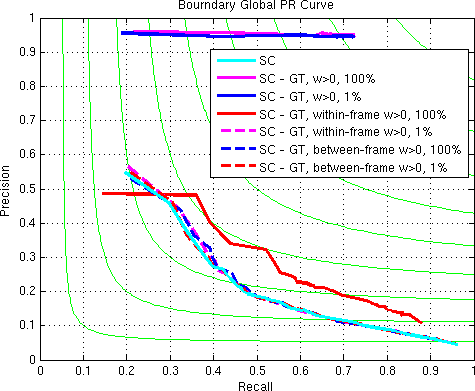
\includegraphics[trim=0cm 0cm 0cm 0.5cm, clip=true, width=0.45\textwidth]{images/connect/2.png}}
%\hfill
\quad
% \subfigure{%
% 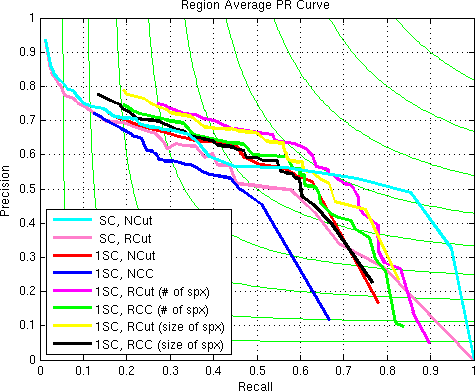
\includegraphics[trim=0cm 0cm 0cm 0.8cm, clip=true, width=0.47\textwidth]{images/basic/3.png}}
\subfigure[VPR]{%
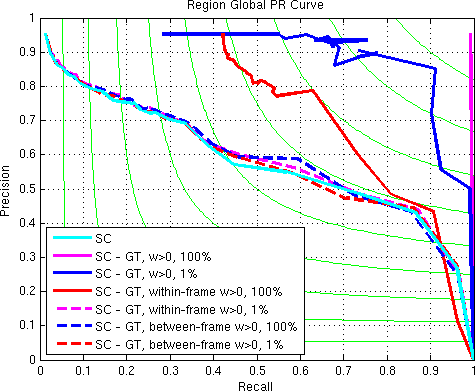
\includegraphics[trim=0cm 0cm 0cm 0.5cm, clip=true, width=0.45\textwidth]{images/connect/4.png}}

\caption[Boundary precision-recall (BPR) and volume precision-recall (VPR) curves for spectral clustering (SC) using true connected components of the affinity matrix as must-links]{
{\bf Boundary precision-recall (BPR) and volume precision-recall (VPR) curves for spectral clustering (SC) using true connected components of the affinity matrix as must-links}.
Here we consider 3 types of connections: within-, between- and within- and between-frame. We merge 1\% or 100\% of all possible connections.}
\label{fig:aff_conn}
\end{figure}
%ltt annot and old
% \begin{large}\begin{tabular}{|l|c|c|c|c|c|c|c|c|c|c|c|}
% \hline
% &\textbf{1}&\textbf{2 }&\textbf{3}&\textbf{4}&\textbf{5}&\textbf{6}&\textbf{7}&\textbf{8}&\textbf{9}&\textbf{10}&\textbf{$>$10}\\\hline
% \textbf{0-0.2}&0.04529&0.03599&0.03121&0.01988&0.01952&0.01585&0.00407&0.00833&0.00000&0.00000&0.00000\\\hline
% \textbf{0.2-0.4}&0.03783&0.02947&0.02596&0.02302&0.02169&0.01898&0.01497&0.01513&0.01257&0.02096&0.01203\\\hline
% \textbf{0.4-0.6}&0.03603&0.02745&0.02160&0.01990&0.01997&0.01629&0.01936&0.01968&0.01676&0.01127&0.01123\\\hline
% \textbf{0.6-0.8}&0.03237&0.02574&0.02263&0.01831&0.01902&0.02071&0.01770&0.02073&0.01399&0.01613&0.01500\\\hline
% \textbf{0.8-0.9}&NaN&0.02724&0.02284&0.02293&0.01953&0.02413&0.02375&0.02672&0.01372&0.00780&0.01365\\\hline
% \textbf{0.9-0.999}&NaN&NaN&NaN&NaN&0.01955&0.02167&0.02475&0.03427&0.01613&0.02163&0.02426\\\hline
% \textbf{1}&0.03426&0.02530&0.03169&0.04221&0.02726&0.03514&0.01351&0.03944&0.00990&0.04065&0.03023\\\hline
% \end{tabular}
% \end{large}

% % all annot
% \begin{large}\begin{tabular}{|l|c|c|c|c|c|c|c|c|}
% \hline
% &\textbf{ltt}&\textbf{aba}&\textbf{abm}&\textbf{stt}&\textbf{sta}&\textbf{stm}&\textbf{w}&\textbf{w-ltt}\\\hline
% \textbf{0-0.2}&0.04206&0.31711&0.47166&0.06834&0.17260&0.15778&0.09492&0.11420\\\hline
% \textbf{0.2-0.4}&0.02916&0.17173&0.41417&0.04375&0.13200&0.07243&0.06711&0.08840\\\hline
% \textbf{0.4-0.6}&0.02270&0.11006&0.34046&0.03562&0.09938&0.08467&0.06409&0.08217\\\hline
% \textbf{0.6-0.8}&0.02012&0.06118&0.27623&0.03120&0.06989&0.07126&0.06569&0.07620\\\hline
% \textbf{0.8-0.9}&0.02051&0.01627&0.17831&0.02580&0.04790&0.08199&0.06495&0.07000\\\hline
% \textbf{0.9-0.999}&0.02283&0.00247&0.02241&0.04465&0.02137&0.04647&0.03441&0.03443\\\hline
% \textbf{1}&0.03153&NaN&NaN&0.16667&0.00006&0.00000&0.00447&0.00007\\\hline
% \end{tabular}
% \end{large}

The conducted experiments indicate a great potential of employing constrained spectral clustering for video segmentation. 
Even a naive integration of low-level features as must-links shows an increase in the performance. However, not all the constraints are correct and the number of merging decisions is quite small. 
Therefore, we came to the idea to learn must-link constraints from the affinities. With a powerful learning method we could find the right combination of features as must-links and avoid the above mentioned problems.
\section{Learning Must-Link Constraints from Affinities}%{Integration of must-link constraints into spectral clustering}
\label{sec:ch4_ML}
In order to learn must-links from the affinity measures we splitted the dataset into 3 parts: training (6 video sequences), validation (4 sequences) and test (13 sequences) set.
The goal is to solve binary classification problem, to predict whether 2 superpixels belong to the same object (positive class) or not (negative class) based on the affinities. 
The training data consists only of similarities of superpixels which belong to the annotated frames and the labels are assigned according to the ground truth.

As a learning method we chose Random Forest (RF), which was introduced by Leo Breiman~\cite{Breiman01}. The algorithm has become very popular recently in computer vision~\cite{KontschiederBBP11,LimZD13,DollarICCV13edges} 
for having good accuracy and low training and testing time, being robust to noise. However, similar to most classifiers, RF can also suffer from the curse of learning from an extremely unbalanced training data. 
As it is constructed to minimize the overall error rate, it will tend to focus more on the prediction accuracy of the majority class, which often results in poor accuracy for the minority class. 

In our case the training set is highly unbalanced, more than 90\% of the data belongs to the positive class.
To alleviate the problem, we propose to use the one-sided sampling technique to randomly down-sample the majority class
and grow each tree on a more balanced dataset.
Recent research~\cite{Drummond03,Breiman04} shows that for the tree classifier artificially making class priors equal either by down-sampling the majority class or over-sampling
the minority class is usually more effective than other approaches, and that down-sampling seems to have an edge over over-sampling. However, down-sampling the majority class may result
in loss of information, as a large part of the majority class is not used. 

For every video sequence we have roughly the 1st, 9th, 10th, 11th, 20th and 30th frame annotated. The affinities which we use in our work (see sec.~\ref{sec:ch3_affinities}) measure the similarity between superpixels in a different
temporal neighbourhood. Therefore for better performance we distinguish 4 types of learning settings based on the temporal connections between superpixels %: within frame, between 1 frame, between 2 frames and between more than 2 frames.
and each type has its own set of features:
\renewcommand{\arraystretch}{1.3}
\begin{center}
\begin{tabular}{|l|l|}
\hline
\textbf{Type}&\textbf{Features}\\\hline
within frame& ABA, ABM, STA, STM\\\hline
between 1 frame& STA, STM, STT\\\hline
between 2 frames& STT, LTT, CTR\\\hline
between $\mathrm{>}$ 2 frames& LTT, CTR\\\hline
\end{tabular} 
\end{center}
We used additional feature CTR - the number of common trajectories which intersect both superpixels, as it was observed in the experiments in the Section~\ref{sec:ch3_aff} that the performance of LTT is more accurate with a sufficient 
number of common trajectories. LTT and CTR are not considered as features for ''between 1 frame`` type because it is much easier for them to achieve high values in the 1 frame neighbourhood and they can bring additional noise 
to the data. It is worth mentioning that for ''between $\mathrm{>}$ 2 frames`` type we do not have the training data for all superpixels in the temporal neighbourhood, e.g. 4 frames apart. On account of that we 
only consider superpixels for which we have the training data, more than 7 frames apart.

In our setting with highly unbalanced data, the overall classification accuracy is not an appropriate measure of performance. A trivial classifier that predicts every case as the majority class can still achieve very high
accuracy. Besides, our goal is to learn must-link constraints without making any mistakes. Therefore we are more interested to have the low number of false positives (FP) and high number of true positives (TP) to make the maximum
of correct must-link decisions.
To evaluate the performance of the algorithm on our data the following measure is used: $\mathrm{|FP|/|FP+TP|}$.

Usually in practice for RF we try to maximize an information gain, the minimum number of samples in a leaf node is set to quite a small value and number of features to sample for each node split
is set to $\mathrm{\sqrt{F}}$ which gives a suboptimal solution, where $\mathrm{F}$ is the dimensionality of the feature space.
The averaged prediction of the individual trees is taken as usual for prediction of the ensemble.
So, the only parameters which are adjusted in a particular application task
are the choice of weak learners, the number of trees in RF and the maximum depth of each tree. In this work as weak learners we use linear binary split functions and conic sections, and the forest size is set to 100 trees, 
which leads to much smoother posteriors and decreases the test error~\cite{Criminisi12}.
We trained RF with various maximum depths of the tree, starting from 2 till 12. % and choose the optimal depth while testing on the validation set. 

In this thesis we use a RF implementation for MATLAB by Stanford Vision Lab. The code is available at \url{https://github.com/karpathy/Random-Forest-Matlab}.
\subsection{Random Forest Classifier Evaluation}
In our application we want to avoid making wrong must-link decisions, therefore we need to find the threshold for the output value of the classifier, which gives the minimum number of false positives and 
the maximum number of true positives. All the optimal parameters, threshold and maximum tree depth, are chosen while testing on the validation set.

Figure~\ref{fig:hist_fp} represents the histograms which show the relation between the number of false positives and percentage of must-link decisions for various tree depths and different types of temporal connections. 
Each bin of the histogram corresponds to a particular threshold of the classifier prediction. %In order to correctly evaluate the result of the learned classifier a graph propagation effect should be taken into account. If several groups of nodes are merged together 
\begin{figure}[htbp]
\centering
% \begin{minipage}[t]{1\textwidth}
% \centering
% \subfigure{%
% 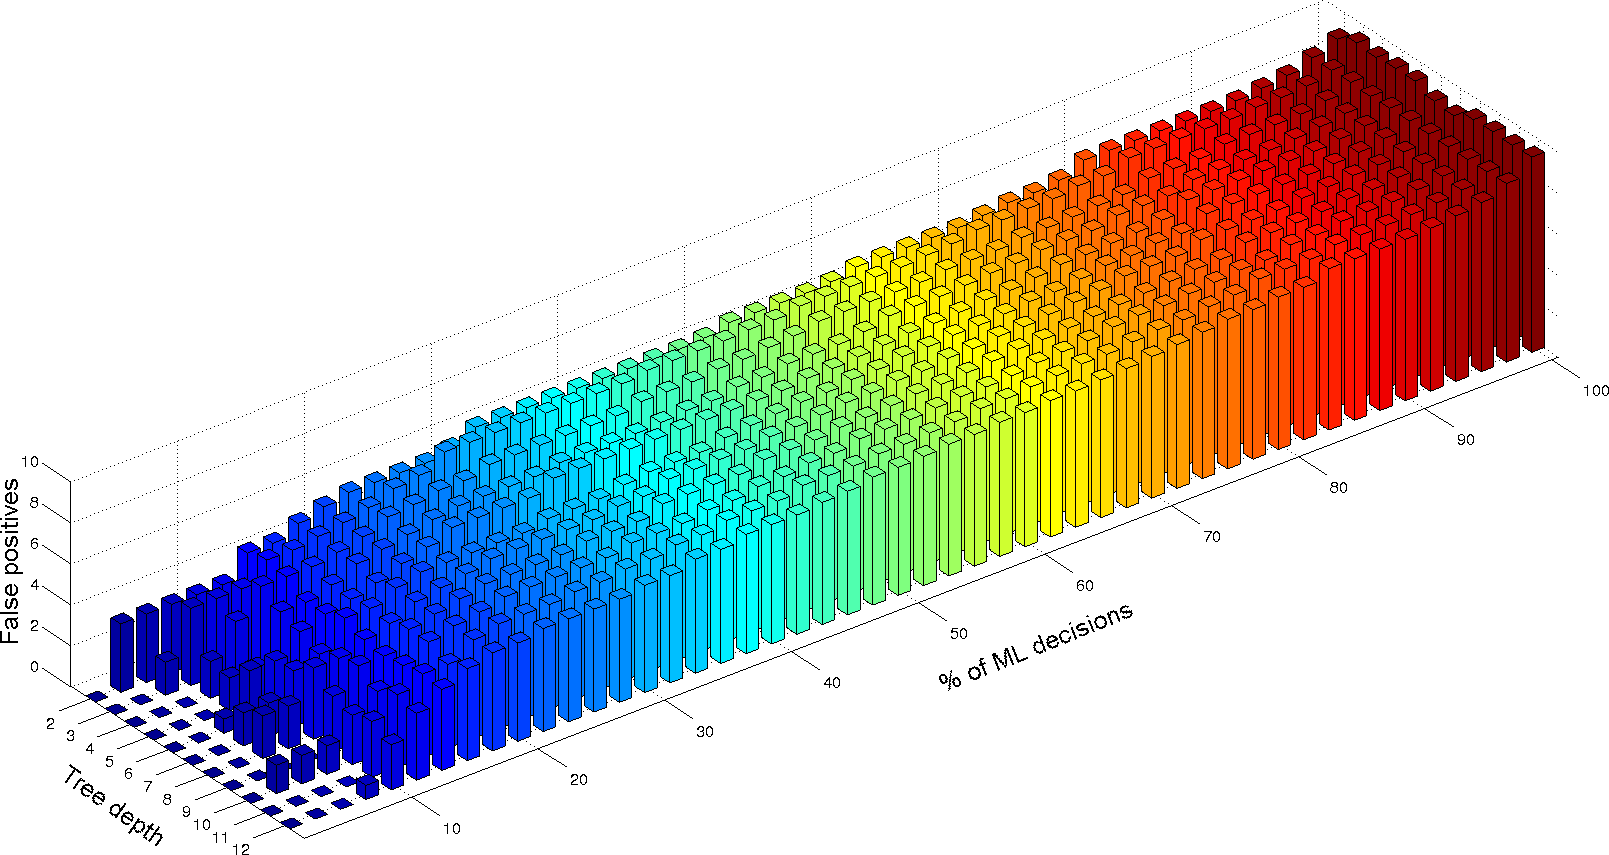
\includegraphics[width=0.48\textwidth]{images/hist_ml/w/fpo.png}}
% \hfill
\subfigure[Within frame]{%
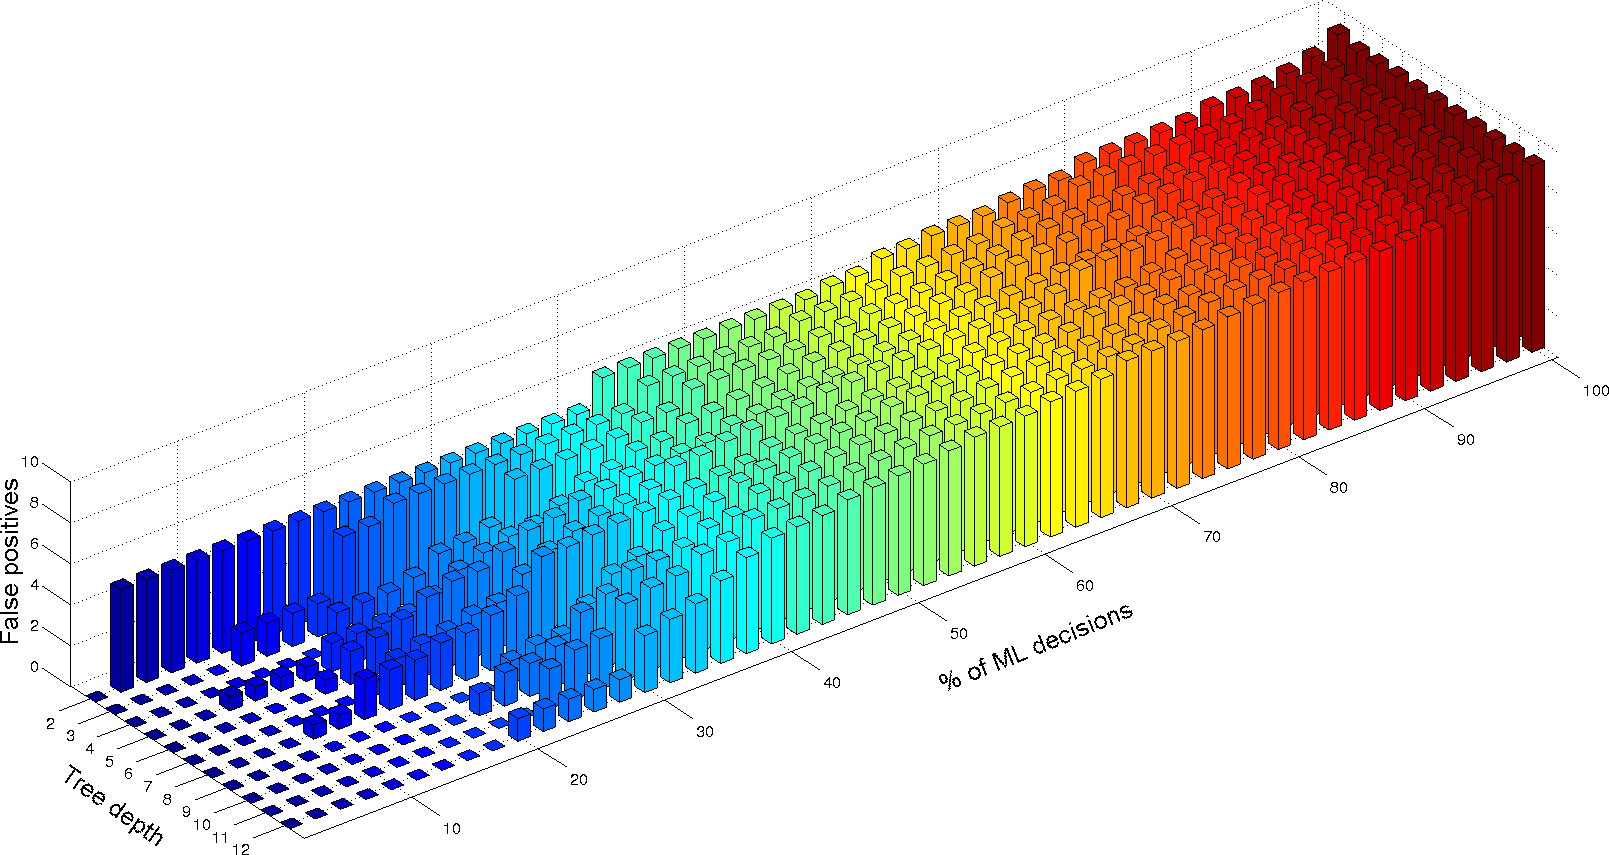
\includegraphics[width=0.48\textwidth]{images/hist_ml/w/fp.png}}
% 
% \footnotesize (a) Within frame
% \end{minipage}
% \begin{minipage}[t]{1\textwidth}
% \centering
% \subfigure{%
% 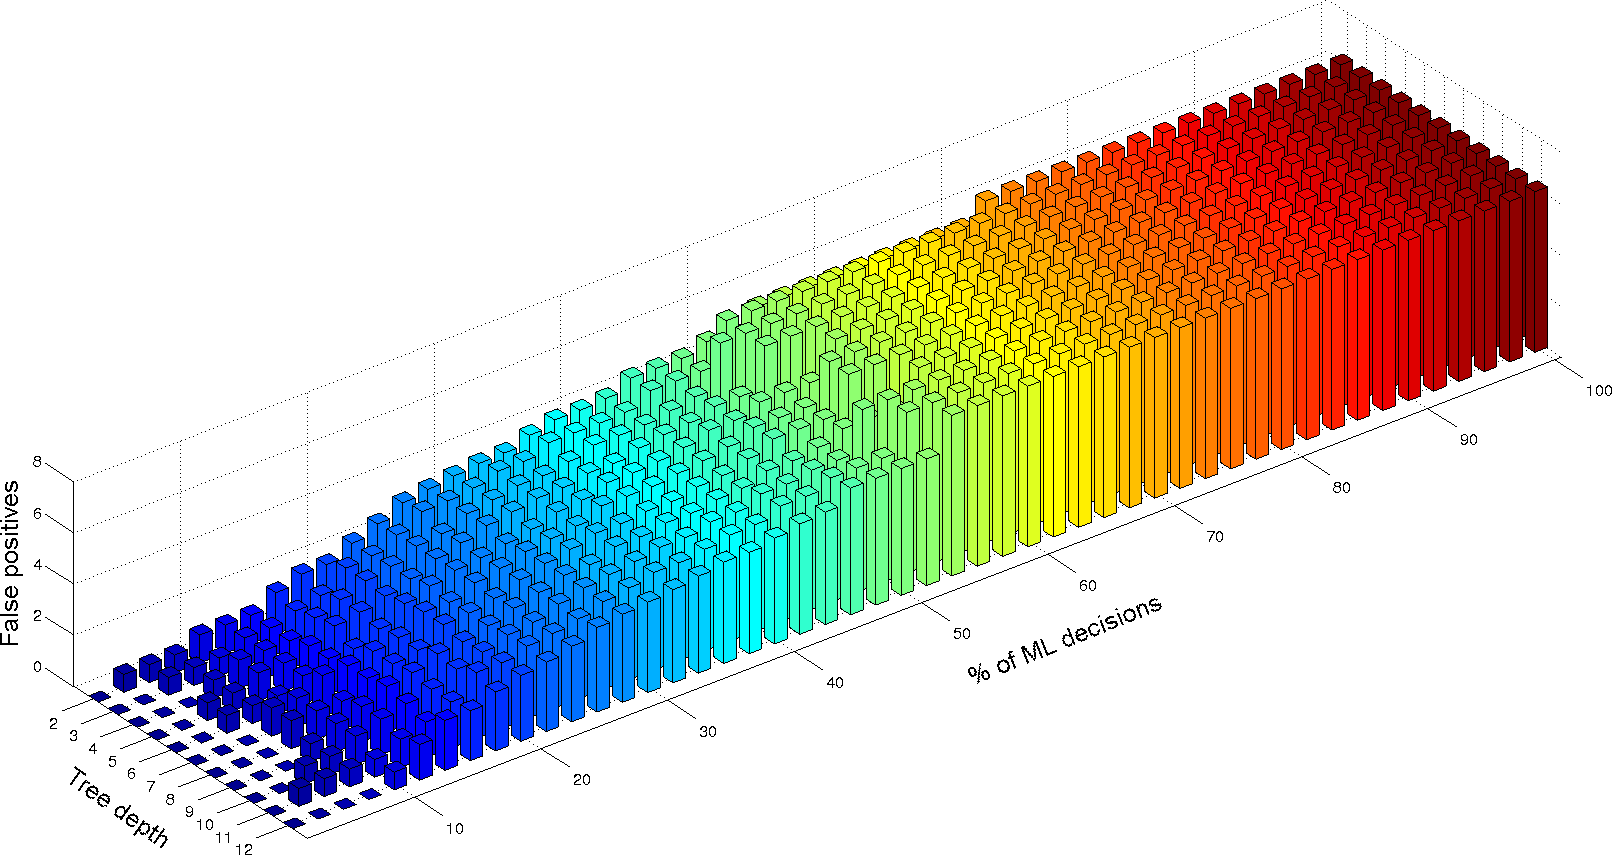
\includegraphics[width=0.48\textwidth]{images/hist_ml/a2/fpo.png}}
\hfill
\subfigure[Between 1 frames]{%
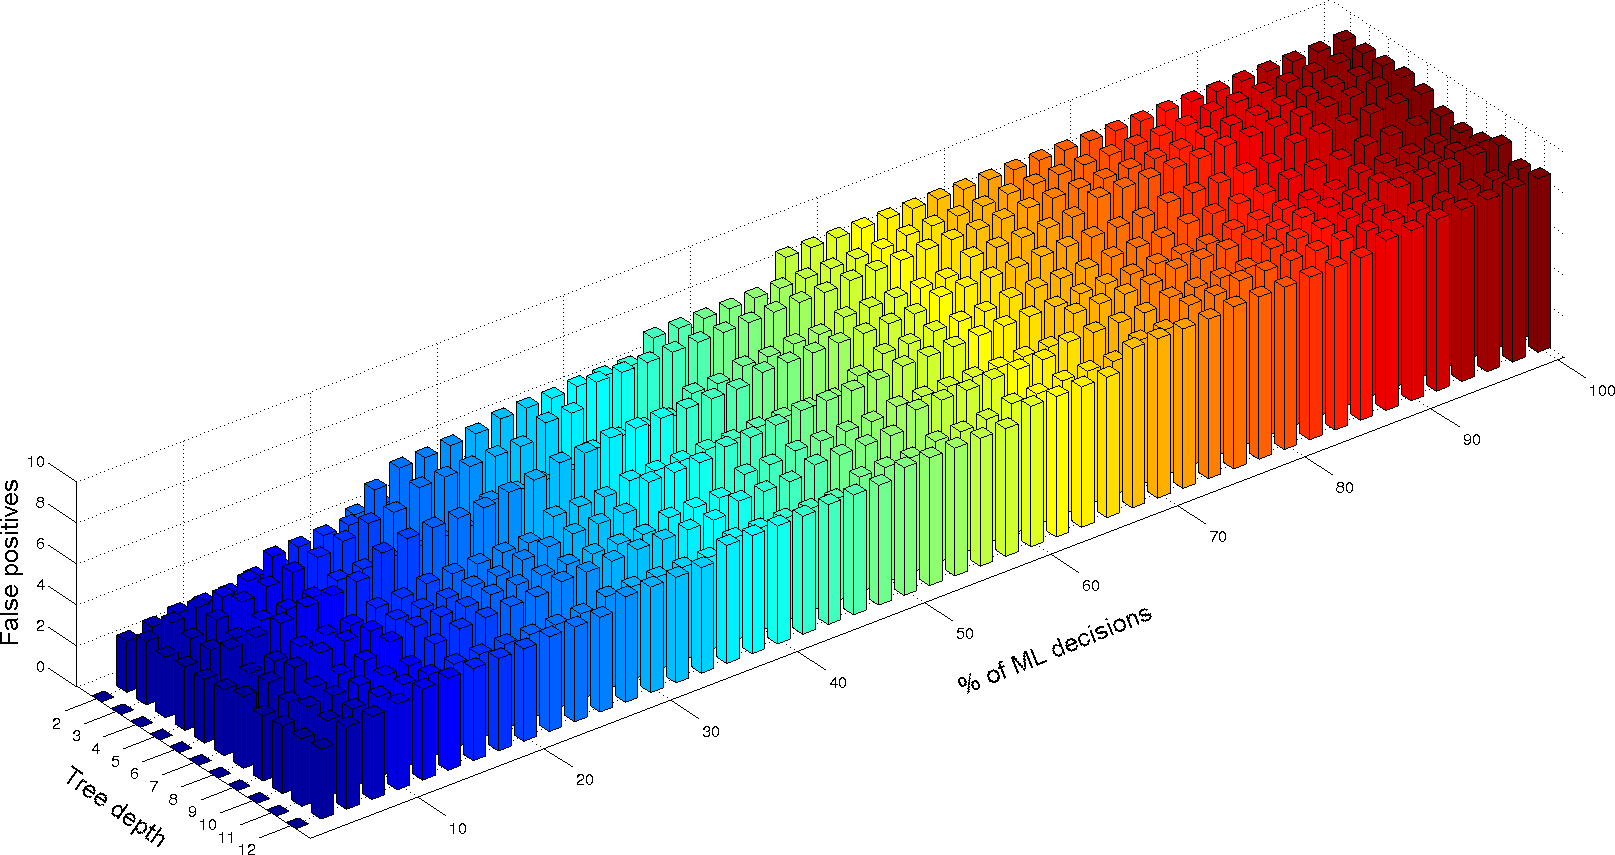
\includegraphics[width=0.48\textwidth]{images/hist_ml/a1/fp.png}}
\hfill
\subfigure[Between 2 frames]{%
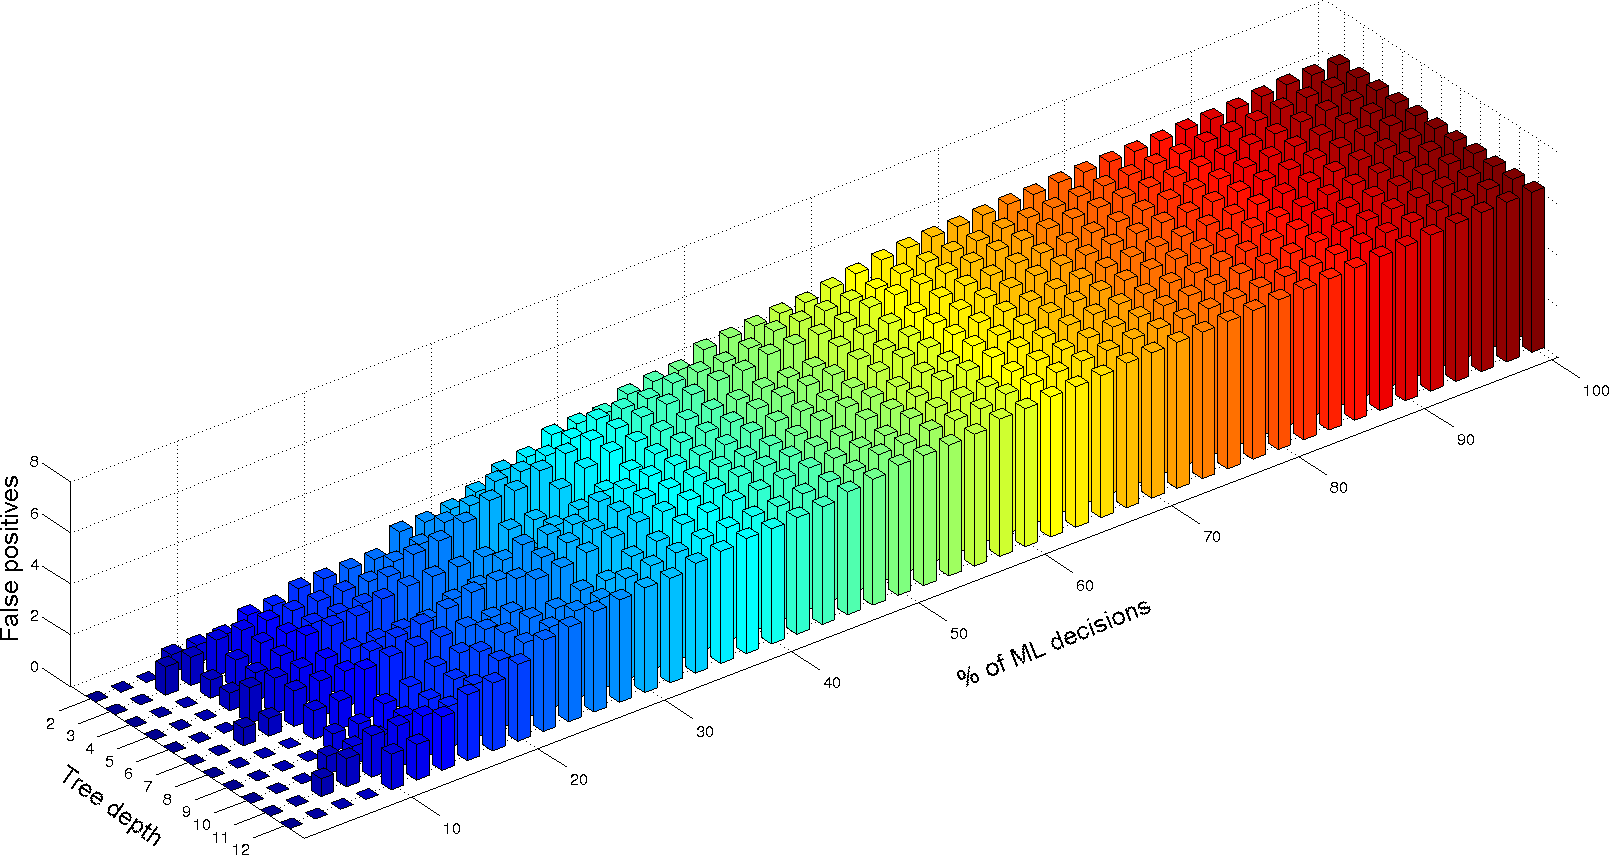
\includegraphics[width=0.48\textwidth]{images/hist_ml/a2/fp.png}}
\hfill
\subfigure[Between $>$ 2 frames]{%
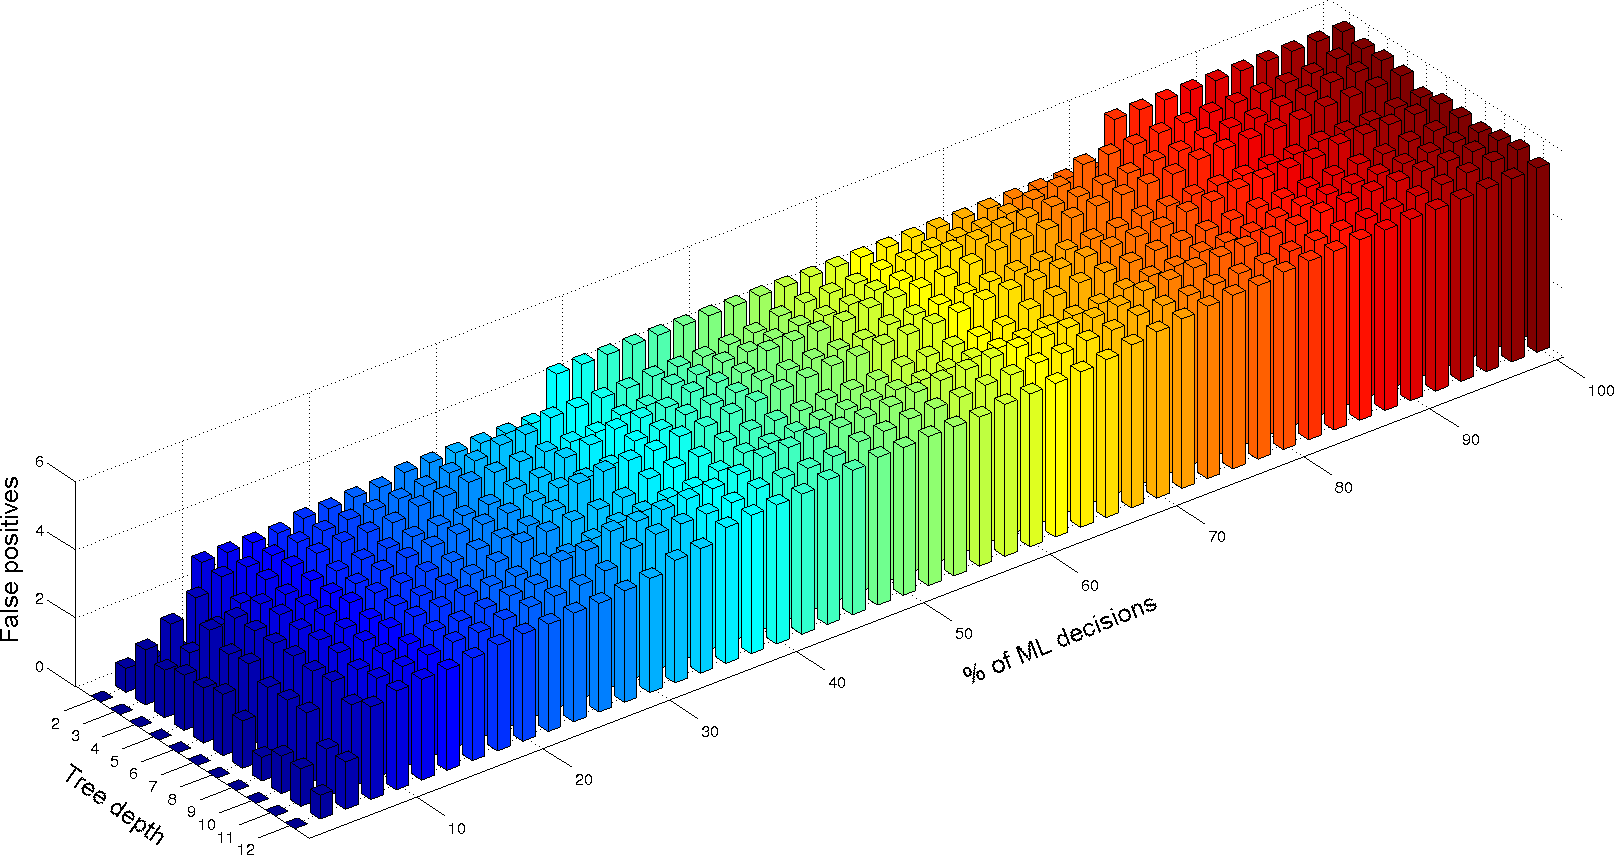
\includegraphics[width=0.48\textwidth]{images/hist_ml/a_2/fp_n.png}}
% 
% \footnotesize (b)Between 2 frames
% \end{minipage}
\caption[Relation between the number of false positives and percentage of must-link decisions]{
{\bf Relation between the number of false positives (in logarithmic scale) and percentage of must-link decisions (ML) for different tree depths and types of temporal connections.}}
\label{fig:hist_fp}
\end{figure}

For each percentage of must-link decisions the optimal tree depth which gives the minimum error rate was found. The results are reported in Figure~\ref{fig:plots_fpr}.
Each point of the curve is coherent with a certain classifier and threshold.
\begin{figure}[htbp]
\centering
\subfigure{%
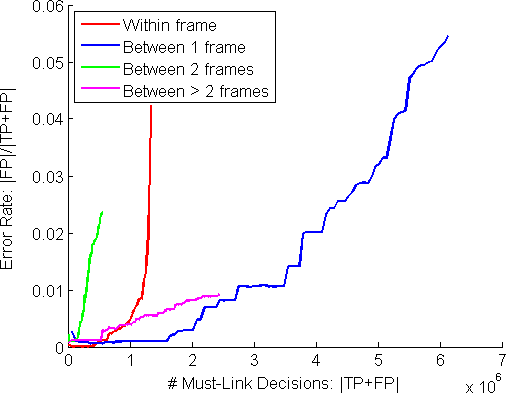
\includegraphics[width=0.45\textwidth]{images/fpr_nML.png}}
\quad
\subfigure{%
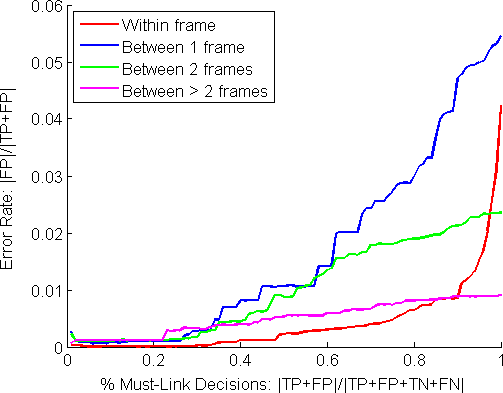
\includegraphics[width=0.45\textwidth]{images/fpr_pML.png}}
 \caption[Relation between the error rate and number or percentage of must-link decisions for different types of temporal connections]{
  {\bf Relation between the error rate and number or percentage of must-link decisions for different types of temporal connections.}}
\label{fig:plots_fpr}
\end{figure}
\newpage
From the plots it can be observed that the dynamic is different depending on the considered temporal neighbourhood. We can afford different number of decisions with the minimum error rate for various types.
The best type is ''within frame``, which is not surprising as all the annotated frames are used for training and the difficulties inherent to video, e.g. illumination changes, are absent here.

Our goal is to choose the best classifier for each type and combined all of them together as a final result. The main question how many false decisions are allowed without loss of the performance.  
Figure~\ref{fig:sc_fp} illustrates the evaluation of video segmentation employing the constrained spectral clustering with learned must-links. The results are aggregated on the test part of the BMDS. 
In this experiment the classifier and the corresponding threshold are chosen 
according to the number of false positives (FP = 0,1,3) which gives the minimum error rate.

It can be seen that even if for individual types we can afford a few errors without a drop in the precision or with a growth of the performance, like for ''within frame``, but the combination of all of them is intricate and leads to much more
incorrect decisions due to the error propagation effect of the graph. If 2 nodes of the graph are merged together, then other nodes which are linked to each of them are influenced too and they should all form one node in the reduced
graph. Therefore even one false link could result in the significant drop of the performance, especially if all types of connections in the graph are considered.

The error propagation effect is illustrated in Figure~\ref{fig:err_eff} for the video sequence ''Marple4`` for ''within frame'' case. It can be observed that a few incorrect must-link decisions can result in the foreground object being
merged to the background even if we only consider one type of connections.
Hence the effect could be much worse when combining all the classifiers for different temporal neighbourhoods and it is better to avoid any mistakes for individual cases. 
For all the following experiments we will choose for each type the optimal tree depth and threshold
of the classifier which yield the maximum number of must-links with error rate equal zero.

\begin{figure}[htbp]
\begin{minipage}[t]{1\textwidth}
\centering
\footnotesize \hfill BPR\hfill \quad
\footnotesize VPR\hfill \hfill
\end{minipage}
\begin{minipage}[t]{1\textwidth}
\centering
\subfigure{%
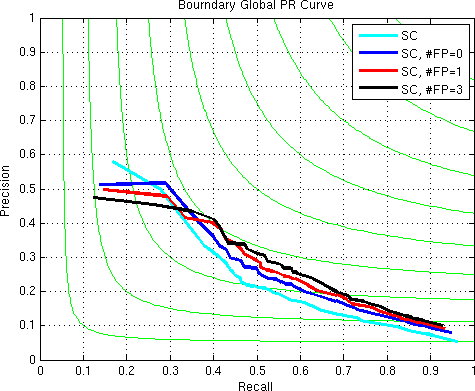
\includegraphics[trim=0cm 0cm 0cm 0.5cm, clip=true, width=0.33\textwidth]{images/RF_propagation_res_2/within/2.png}} 
\quad
\subfigure{%
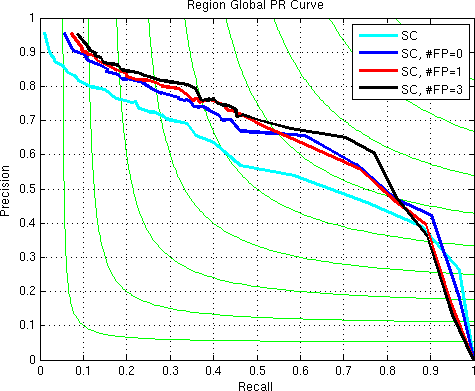
\includegraphics[trim=0cm 0cm 0cm 0.5cm, clip=true, width=0.33\textwidth]{images/RF_propagation_res_2/within/4.png}} 

\footnotesize (a) Within frame
\end{minipage}
\begin{minipage}[t]{1\textwidth}
\centering
\subfigure{%
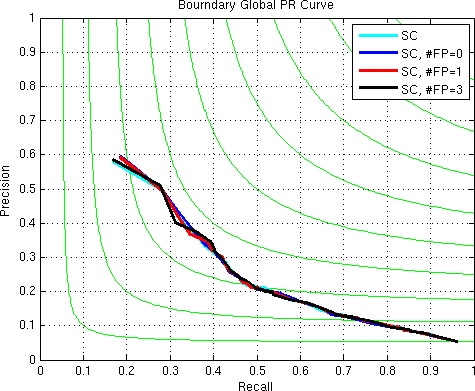
\includegraphics[trim=0cm 0cm 0cm 0.5cm, clip=true, width=0.33\textwidth]{images/RF_propagation_res_2/across1/2.png}} 
\quad
\subfigure{%
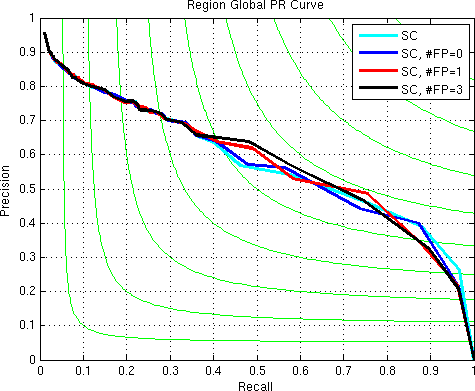
\includegraphics[trim=0cm 0cm 0cm 0.5cm, clip=true, width=0.33\textwidth]{images/RF_propagation_res_2/across1/4.png}} 

\footnotesize (b) Between 1 frame
\end{minipage}
\begin{minipage}[t]{1\textwidth}
\centering
\subfigure{%
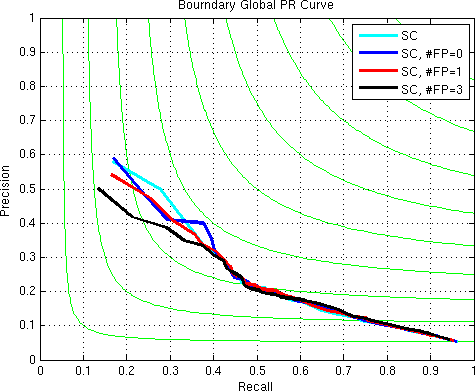
\includegraphics[trim=0cm 0cm 0cm 0.5cm, clip=true, width=0.33\textwidth]{images/RF_propagation_res_2/across2/2.png}} 
\quad
\subfigure{%
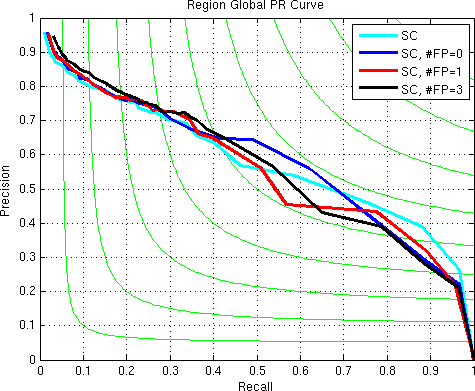
\includegraphics[trim=0cm 0cm 0cm 0.5cm, clip=true, width=0.33\textwidth]{images/RF_propagation_res_2/across2/4.png}} 

\footnotesize (c) Between 2 frames
\end{minipage}
\begin{minipage}[t]{1\textwidth}
\centering
\subfigure{%
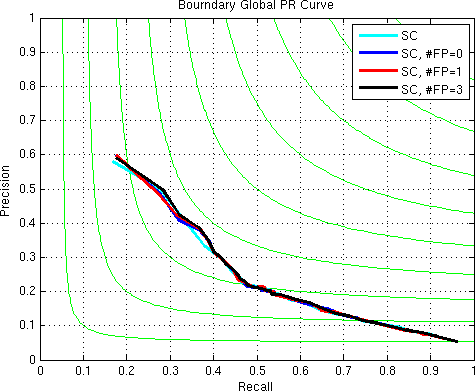
\includegraphics[trim=0cm 0cm 0cm 0.5cm, clip=true, width=0.33\textwidth]{images/RF_propagation_res_2/across>n/2.png}} 
\quad
\subfigure{%
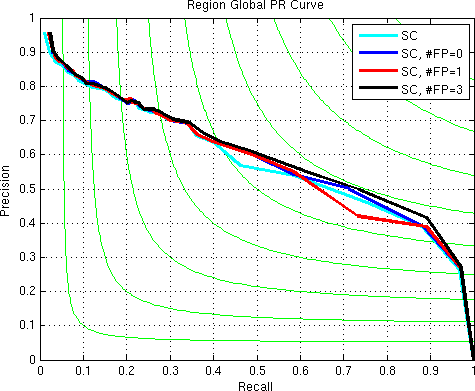
\includegraphics[trim=0cm 0cm 0cm 0.5cm, clip=true, width=0.33\textwidth]{images/RF_propagation_res_2/across>n/4.png}} 

\footnotesize (d) Between more than 2 frames
\end{minipage}
\begin{minipage}[t]{1\textwidth}
\centering
\subfigure{%
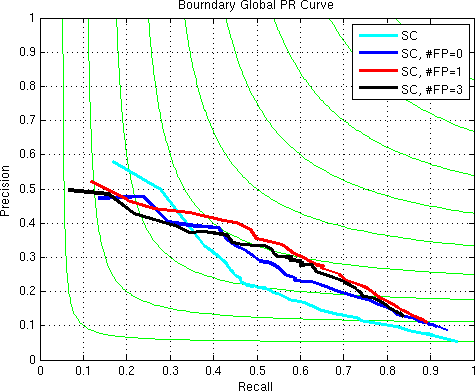
\includegraphics[trim=0cm 0cm 0cm 0.5cm, clip=true, width=0.33\textwidth]{images/RF_propagation_res_2/all_across_>n/2.png}} 
\quad
\subfigure{%
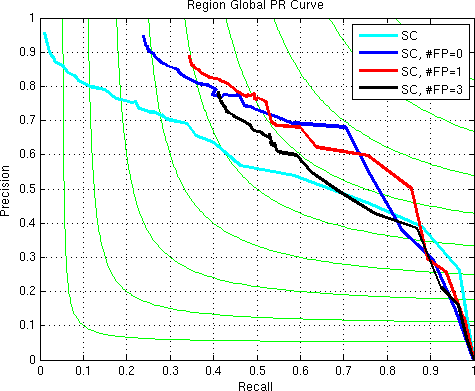
\includegraphics[trim=0cm 0cm 0cm 0.5cm, clip=true, width=0.33\textwidth]{images/RF_propagation_res_2/all_across_>n/4.png}} 

\footnotesize (e) All
\end{minipage}

\caption[Boundary precision-recall and volume precision-recall curves for spectral clustering with choosing RF classifier according to the number of false positives equal 0,1,3]{
{\bf Boundary precision-recall (BPR) and volume precision-recall (VPR) curves for spectral clustering with choosing RF classifier according to the number of false positives (FP = 0,1,3).}}
% We consider 4 types of connections: within frame, 
%between 1 frame, between 2 frames, between more than 2 frames and all of them combined together.}
\label{fig:sc_fp}
\end{figure}
\begin{figure}[htbp]
\centering
% \begin{minipage}[t]{0.1\textwidth}
% \begin{picture}(320,1)
% \put(35,45){\vector(0,-1){320}}
% \end{picture}
% \end{minipage}
% \begin{minipage}[t]{0.9\textwidth}

\includegraphics[width=0.8\textwidth]{images/errors/Marplefour_4_0.png}
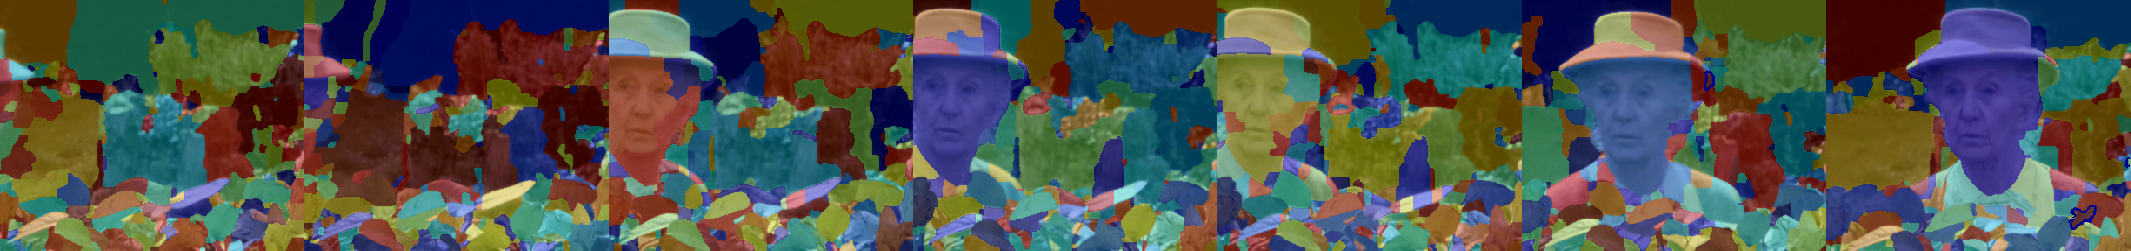
\includegraphics[width=0.8\textwidth]{images/errors/Marplefour_6_3.png}
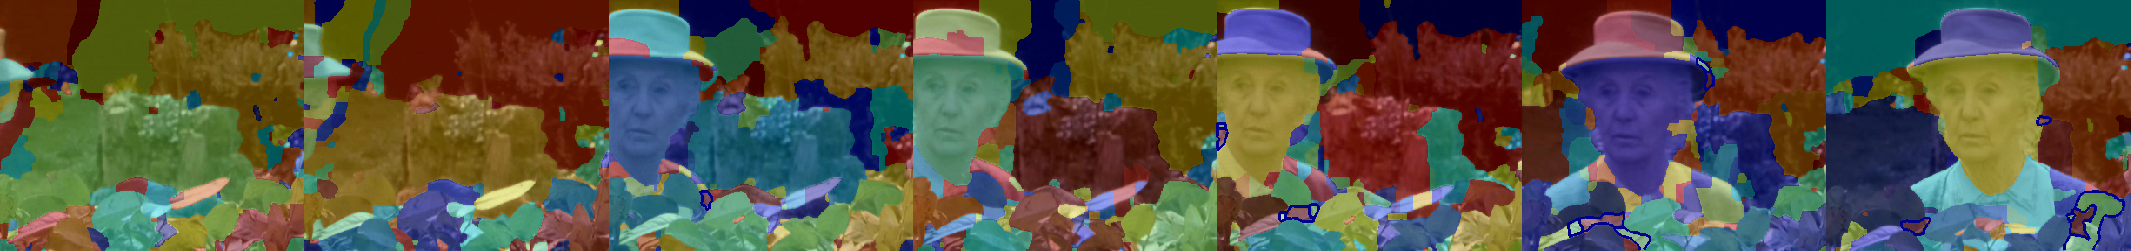
\includegraphics[width=0.8\textwidth]{images/errors/Marplefour_7_14.png}
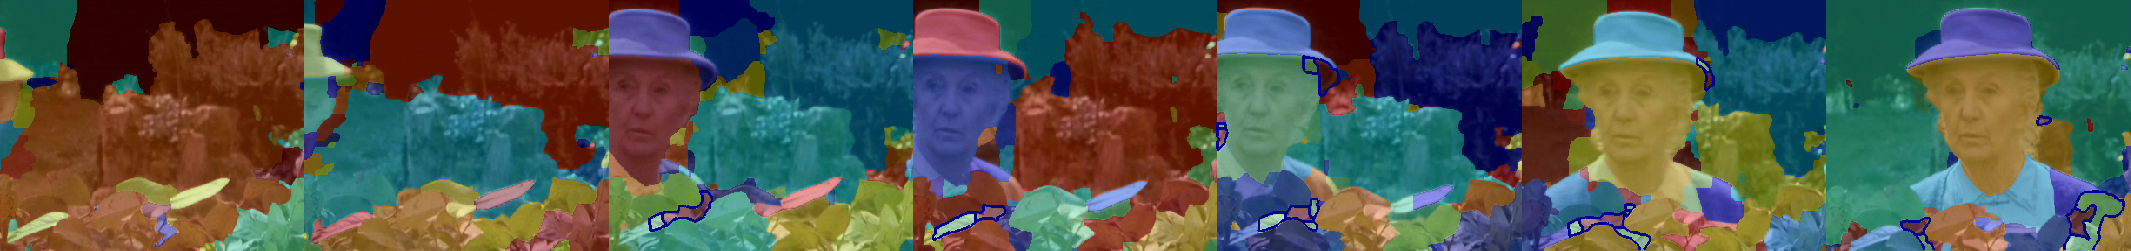
\includegraphics[width=0.8\textwidth]{images/errors/Marplefour_10_20.png}
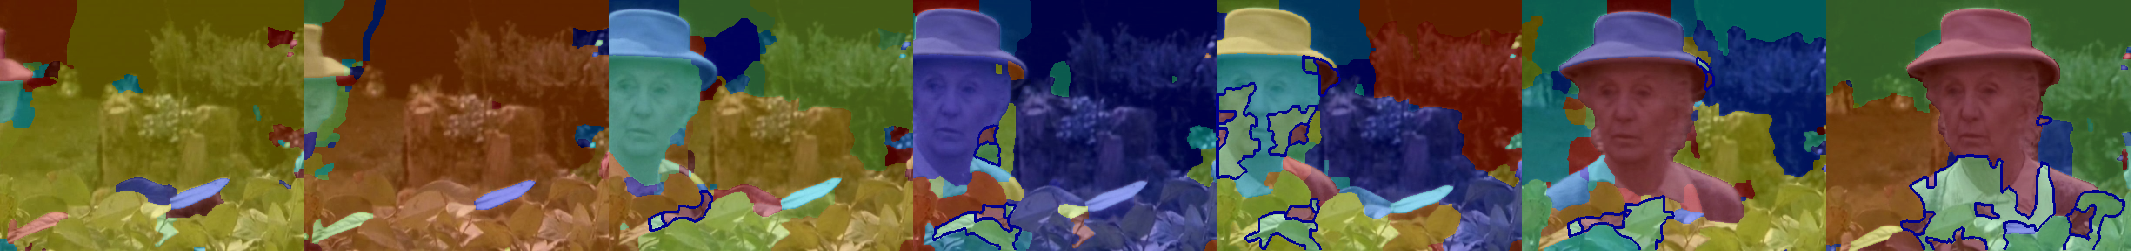
\includegraphics[width=0.8\textwidth]{images/errors/Marplefour_12_29.png}
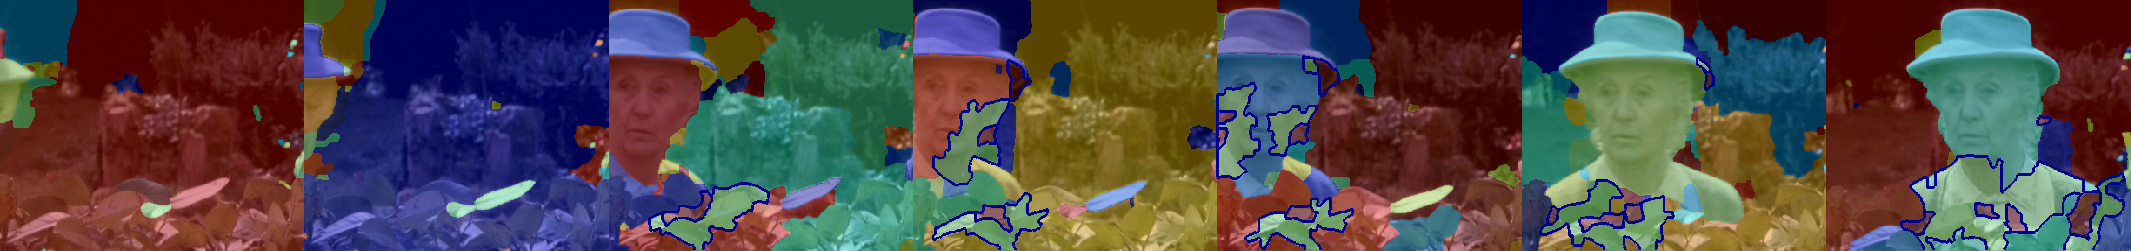
\includegraphics[width=0.8\textwidth]{images/errors/Marplefour_13_35.png}
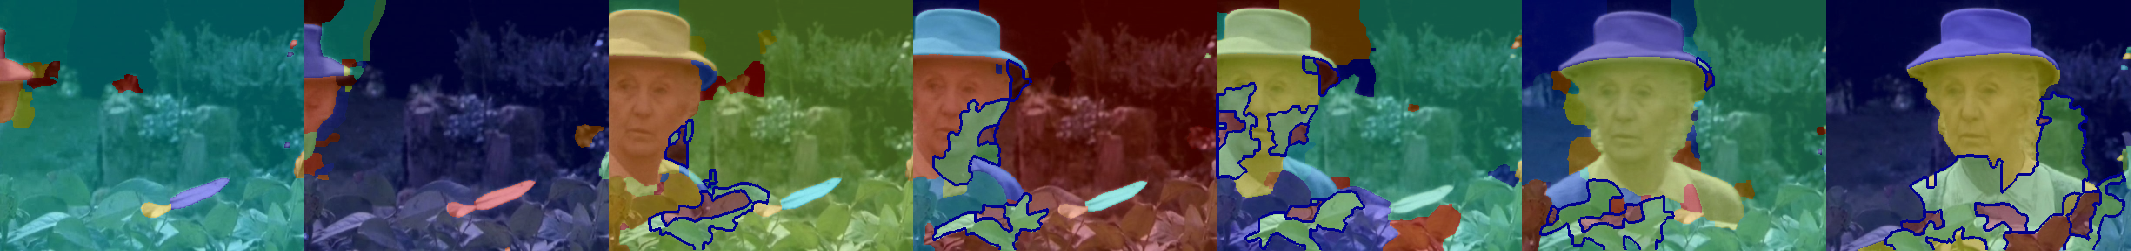
\includegraphics[width=0.8\textwidth]{images/errors/Marplefour_15_45.png}
%\end{minipage}
\caption[Example of error propagation effect]{
{\bf Example of error propagation effect.} The number of false positives grows from 0 to 45.
The red area indicates superpixels incorrectly merged together by the classifier prediction and the green area shows the propagation effect of the occurred errors.}
\label{fig:err_eff}
\end{figure}

\subsection{Segmentation Results for Spectral Clustering with Learned Must-Link Constraints}
In this section video segmentation results with constrained spectral clustering are presented.
Figure~\ref{fig:sc_ML_res} illustrates BPR and VPR curves: first we evaluate the performance of the individual cases to identify which contributes the most (a), then a combination of two types (b) and all minus one type (c)
to determine the set providing best overall performance. Numerical results are presented in Table~\ref{tab:ml_comparison}.

The first two plots (a) report the results of the individual types compared to the performance when using all cases. The most contributory is ''within frame`` type. All other ''between frame`` types provide comparable results.

The second two plots (b) reveal more insight which ''between frame'' type is the most beneficial combined with ``within frame''. It can be observed that ``between $>$ 2 frames`` outperforms ''between 1 frame`` type, but 
loses to ''between 2 frames`` in lower segmentation levels. Note the drop in the precision for ''within + between 2 frames`` for a small number of clusters. 

The last plots (c) show which types are essential to obtain overall best performance when combined. For this the results of all when taking out individual cases are compared. The significant drop in the performance
for ''all minus within frame`` is observed, both for boundary and volume metric. For this particular case the results are even worse than for the method~\cite{GalassoCS12}. The BPR and VPR curves are less altered by removing one of the ''between frame`` types. 
It can be seen that by taking out ''between 2 frames`` the performance is improved for higher segmentation levels and vice versa for a bigger number of clusters.

One can observe that the combination of all types together provides the best result and all sets which include ''within frame`` type outperform the method of~\cite{GalassoCS12}.
\begin{figure}[htbp]
% \begin{minipage}[t]{1\textwidth}
%  \centering
% \hfill \hfill \hfill
% \footnotesize $\mathrm{LTT\geq 0.9}$
% \hfill \hfill \hfill
% \footnotesize $\mathrm{(STA=1)\cup(STM=1)}$
% \hfill \hfill \hfill
% \footnotesize $\mathrm{ABA\geq 0.9}$
% \hfill  \hfill \hfill 
% \end{minipage}
\begin{minipage}[t]{1\textwidth}
\centering
\footnotesize BPR

\hfill \hfill    
\subfigure{%
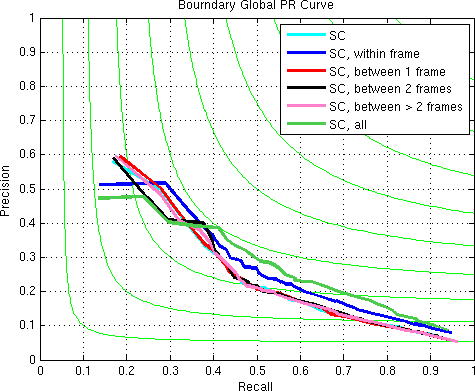
\includegraphics[trim=0cm 0cm 0cm 0.5cm, clip=true, width=0.3\textwidth]{images/res_rf/2.png}} 
\hfill  
\subfigure{%
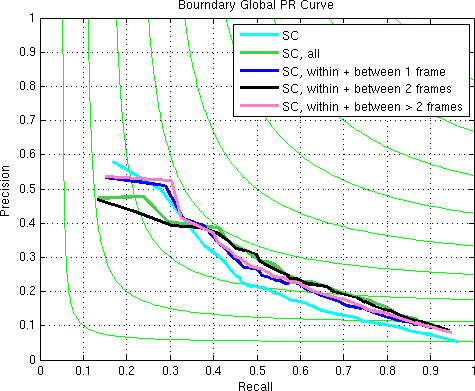
\includegraphics[trim=0cm 0cm 0cm 0.5cm, clip=true, width=0.3\textwidth]{images/res_rf/2_wb.png}} 
\hfill 
\subfigure{%
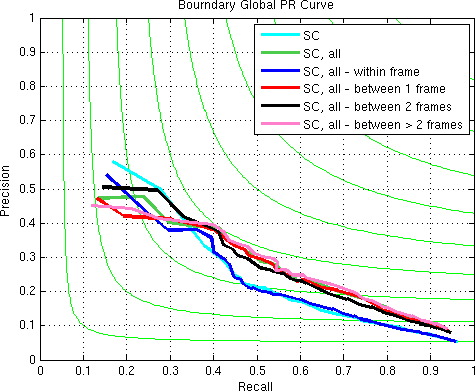
\includegraphics[trim=0cm 0cm 0cm 0.5cm, clip=true, width=0.3\textwidth]{images/res_rf/2_am.png}} 
\hfill   \hfill
\end{minipage}
\begin{minipage}[t]{1\textwidth}
\centering
\footnotesize VPR

\setcounter{subfigure}{0}
\hfill \hfill   
\subfigure[]{%
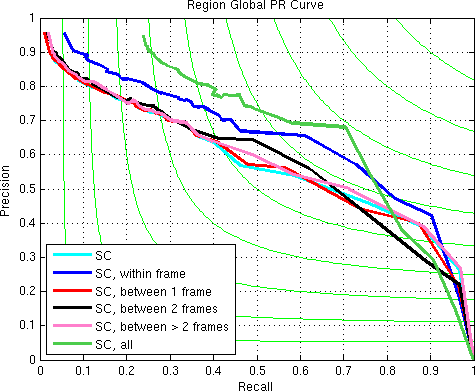
\includegraphics[trim=0cm 0cm 0cm 0.5cm, clip=true, width=0.3\textwidth]{images/res_rf/4.png}} 
\hfill  
\subfigure[]{%
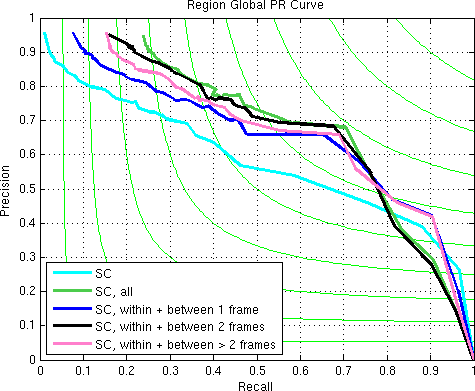
\includegraphics[trim=0cm 0cm 0cm 0.5cm, clip=true, width=0.3\textwidth]{images/res_rf/4_wb.png}} 
\hfill 
\subfigure[]{%
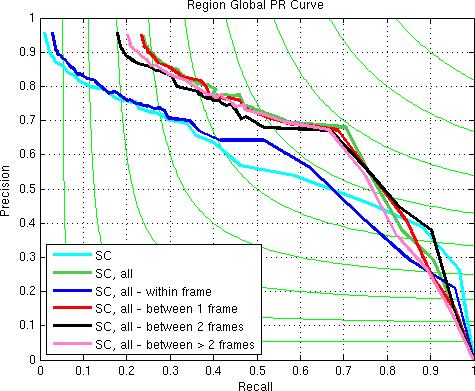
\includegraphics[trim=0cm 0cm 0cm 0.5cm, clip=true, width=0.3\textwidth]{images/res_rf/4_am.png}} 
\hfill   \hfill
\end{minipage}

\caption[Boundary precision-recall and volume precision-recall curves for spectral clustering using different types of connections as must-links]{
{\bf Boundary precision-recall (BPR) and volume precision-recall (VPR) curves for spectral clustering (SC) using different types of connections as must-links.} We consider 4 types of connections: within frame, 
between 1 frame, between 2 frames, between more than 2 frames, all of them combined together, within plus one of the between frames and all minus one type.}
\label{fig:sc_ML_res}
\end{figure}

\begin{table}[htbp]
\renewcommand{\arraystretch}{1.15}
\centering
\scriptsize
%\sffamily
\begin{tabular}{|l||c|c|c||c|c|c||}
\hline 
\multirow{2}{*}{\textbf{Method}} & \multicolumn{3}{c||}{\textbf{BPR}} & \multicolumn{3}{c||}{\textbf{VPR}}\\
\cline{2-7}
& \textbf{ODS}  & \textbf{OSS} & \textbf{AP}
& \textbf{ODS} & \textbf{OSS} & \textbf{AP}\\
\hline
\hline
\textbf{SC} & 0.37 & 0.39 & 0.24 & 0.57 &0.72 & 0.59 \\
\hline \hline
\textbf{SC, within frame} & 0.38 & 0.43 & 0.26 & 0.64 & 0.75 & 0.66\\
\hline
\textbf{SC, between 1 frame} & 0.37 & 0.39 & 0.24 & 0.57 & 0.74 & 0.58\\
\hline
\textbf{SC, between 2 frames} & 0.39 & 0.41 & 0.24 & 0.59 & 0.74 & 0.59\\
\hline
\textbf{SC, between $>$ 2 frames} & 0.37 & 0.42 & 0.24 & 0.59 & 0.73 & 0.60 \\
\hline
\textbf{SC, all} & \textbf{0.40} & \textbf{0.45} & 0.26 & \textbf{0.69} & \textbf{0.77} & \textbf{0.69} \\
\hline
\hline
\textbf{SC, within + between 1 frame} & 0.38 & 0.43 & 0.26 & 0.66 & 0.74 & 0.67 \\
\hline
\textbf{SC, within + between 2 frames} & 0.39 & 0.44 & 0.26 & 0.68 & 0.76 & 0.68 \\
\hline
\textbf{SC, within + between $>$ 2 frames} & 0.38 & 0.42 & \textbf{0.27} & 0.67 & 0.75 & 0.68 \\
\hline
\hline
\textbf{SC, all - within frame} & 0.37 & 0.40 & 0.23 & 0.59 & 0.73 & 0.58 \\
\hline
\textbf{SC, all - between 1 frame} & 0.39 & 0.44 & 0.26 & 0.68 & 0.75 & \textbf{0.69} \\
\hline
\textbf{SC, all - between 2 frames} & 0.39 & 0.42 & 0.26 & 0.67 & 0.76 & \textbf{0.69} \\
\hline
\textbf{SC, all - between $>$ 2 frames} & \textbf{0.40} & 0.44 & \textbf{0.27} & 0.67 & 0.75 & 0.67 \\
\hline
\end{tabular}
 \caption{{\bf Numerical comparison of the results using different types of connections as must-links.} 
The table shows aggregate measures (ODS, OSS, AP) for boundary precision-recall (BPR) and volume precision-recall (VPR) on the test set of the BMDS.}
\label{tab:ml_comparison}
\end{table}

By integrating must-link constraints the reduced graph is constructed with 
much bigger temporal superpixels. As it can be seen from the plots in Figure~\ref{fig:sc_ML_res}, where the last point on VPR (top-left corner) curves indicates the results of 
the initial superpixelization of the algorithm, there is no big drop in the precision, but a crucial increase in the recall is observed. Hence with our model we can extract bigger superpixels without merging objects and
these oversegmentation improves the overall performance of the algorithm.

The quantitative results are supported by the qualitative results. Figure~\ref{fig:spx_res} illustrates superpixelization before (1st row) and after (2nd row) merging superpixels based on learned must-links for 2 video sequences 
''Marple7'' and ``Cars10''. Note that superpixels obtained by our approach mostly accurately capture object boundaries. Moreover, the number of superpixels is significantly decreased, 
thus the runtime and memory consumption are also reduced. These results clearly show the potential of our proposed model for the extraction of superpixels for video segmentation.
% 
% \begin{figure}[ht!]
% \centering
% \subfigure{%
% 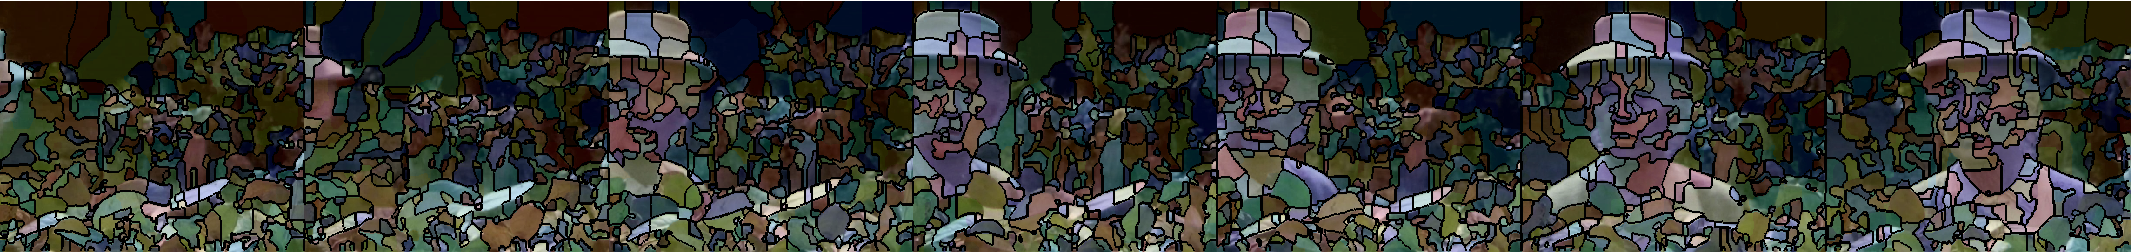
\includegraphics[width=\textwidth]{images/all_vis/M4_old.png}}
% \subfigure{%
% 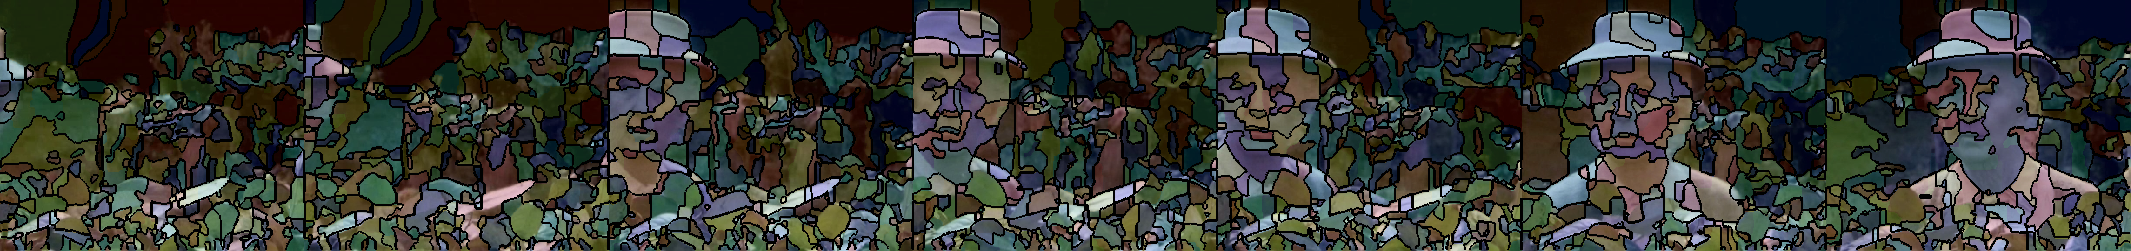
\includegraphics[width=\textwidth]{images/all_vis/M4.png}}
% \subfigure{%
% 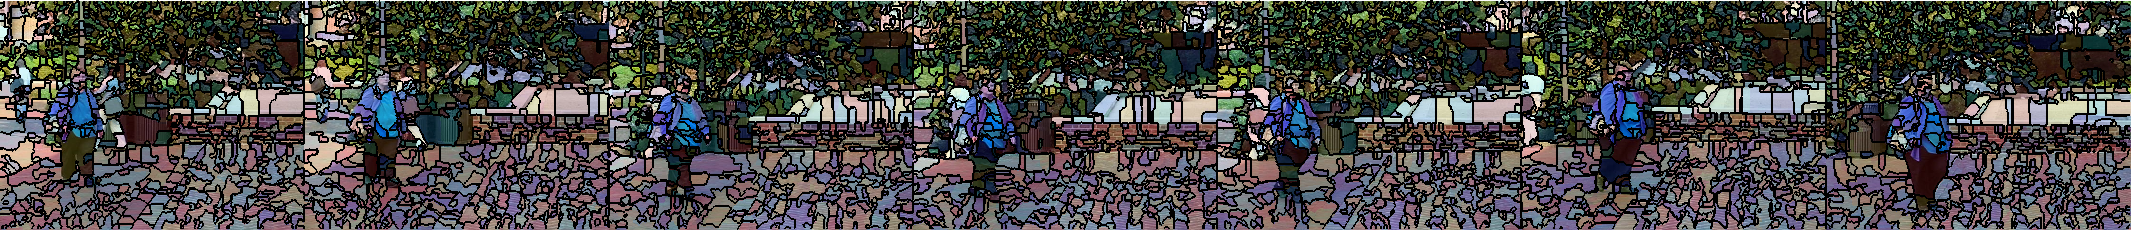
\includegraphics[width=\textwidth]{images/all_vis/P2_old.png}}
% \subfigure{%
% 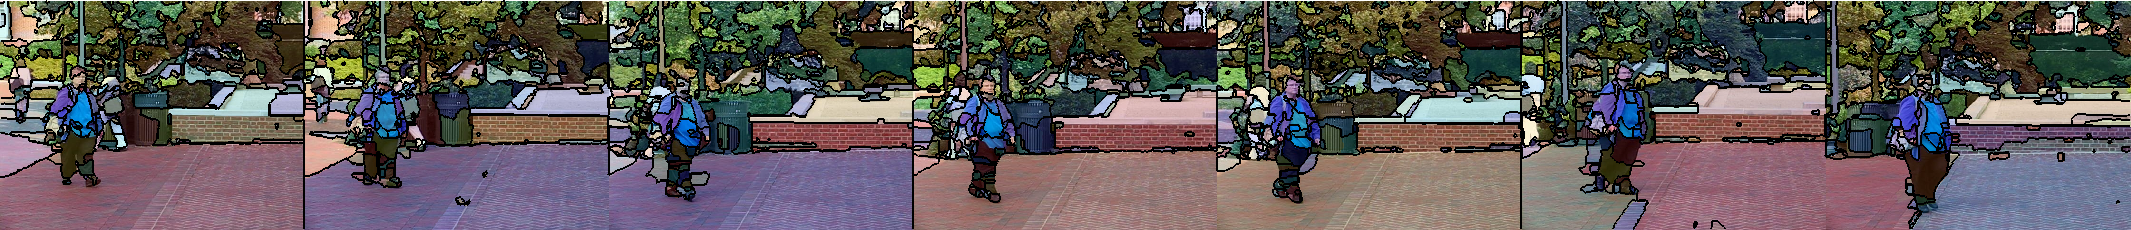
\includegraphics[width=\textwidth]{images/all_vis/P2.png}}
%  \caption[Superpixelization results before and after merging with learned must-links for the video sequences ''Marple4'' and ``People2'']{
%   {\bf Superpixelization results before and after merging with learned must-links for the video sequences ''Marple4'' and ``People2''}.}
% \label{fig:seg_res_C1}
% \end{figure}
\begin{figure}[htbp]
\centering
\subfigure{%
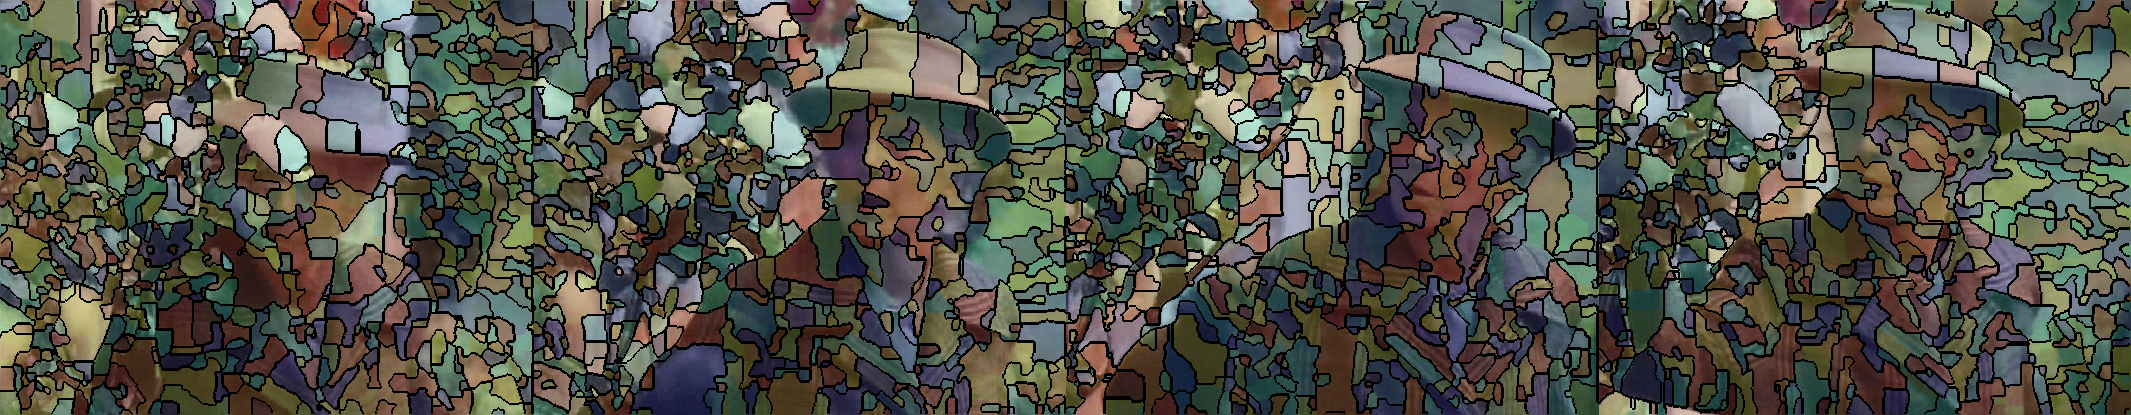
\includegraphics[width=0.65\textwidth]{images/M7_old.png}}
\subfigure{%
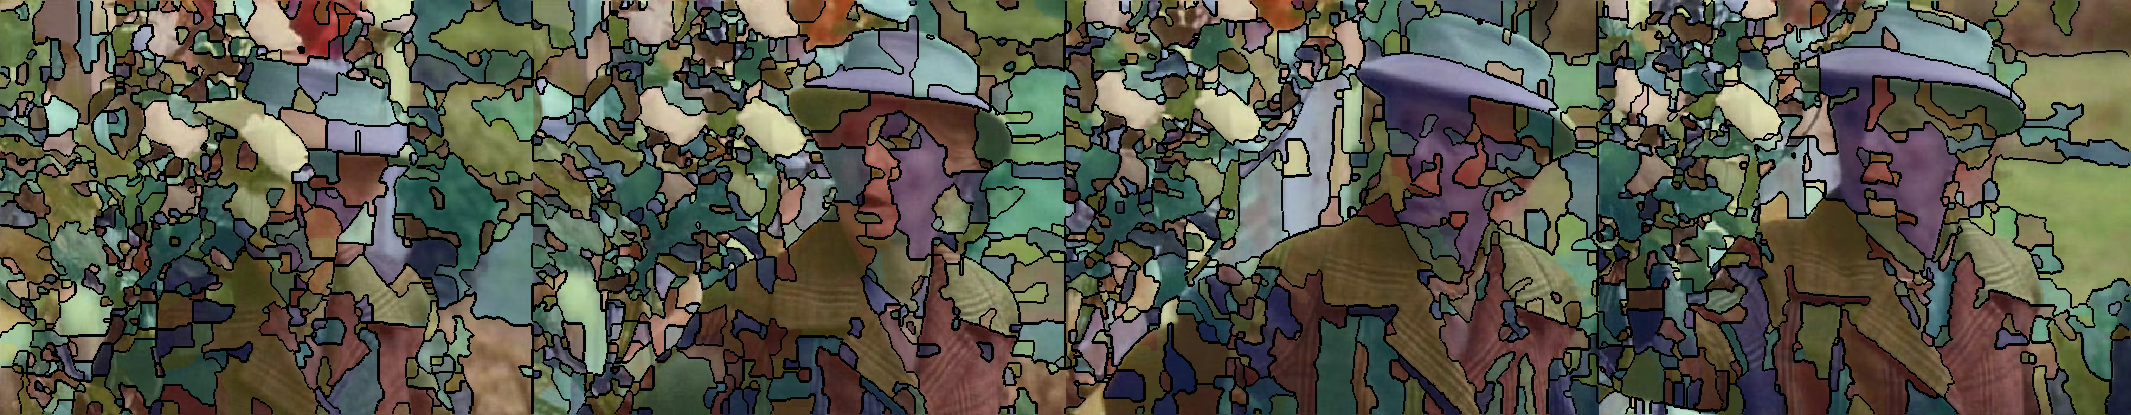
\includegraphics[width=0.65\textwidth]{images/M7.png}}
\subfigure{%
\includegraphics[width=0.65\textwidth]{images/C10_old.png}}
\subfigure{%
\includegraphics[width=0.65\textwidth]{images/C10.png}}
 \caption[Superpixelization results before and after merging with learned must-links for the video sequences ''Marple7'' and ``Cars10'']{
  {\bf Superpixelization results before and after merging with learned must-links for the video sequences ''Marple7'' and ``Cars10''.}}
\label{fig:spx_res}
\end{figure}

We report the qualitative segmentation results in Figure~\ref{fig:seg_res_sc}, comparing our proposed algorithm to the method~\cite{GalassoCS12}.
The clear advantage of our approach is the limited label leakage: integrating must-link constraints enables coarser superpixels adherent to object boundaries, 
which capture better motion and appearance self-contained within the objects. The affinities over larger superpixels might be more beneficial, they allow to distinguish the homogeneous areas of foreground and background.  

Figure~\ref{fig:seg_res_sc_bad} shows additional video segmentations. It illustrates some examples where our approach performs a little bit worse than the method~\cite{GalassoCS12} and reports failure cases for both methods.
For video sequences ``Marple8'' and ``Marple3'' the proposed algorithm needs more clusters to correctly segment the foreground object opposed to the approach~\cite{GalassoCS12}.
Video sequences ``Marple6'', ``Marple9'' and ``Marple10'' represent difficult cases where both methods fail to correctly segment objects. For ``Marple9'' women hardly move, so it is wrongly segmented due to the misleading
appearance differences. In ``Marple6'' the person is not segmented even for high number of clusters, as he does not move and the appearance is not discriminative enough. In ``Marple10'' there is little motion and the person is
occluded.
\renewcommand*{\thesubfigure}{}
\begin{figure}[htbp]
\centering
\begin{minipage}[t]{1\textwidth}
\centering
\footnotesize Cars5%, 3 clusters

\subfigure{%
\includegraphics[width=0.4\textwidth]{images/qual_res/C5_3_old.png}}
\subfigure{%
\includegraphics[width=0.4\textwidth]{images/qual_res/C5_3.png}}
\end{minipage}
\begin{minipage}[t]{1\textwidth}
\centering
\footnotesize Cars3%Tennis, 3 clusters

\subfigure{%
\includegraphics[width=0.4\textwidth]{images/qual_res/C3_6_old.png}}
\subfigure{%
\includegraphics[width=0.4\textwidth]{images/qual_res/C3_5.png}}
\end{minipage}
\begin{minipage}[t]{1\textwidth}
\centering
\footnotesize Marple2%, 2 clusters

\subfigure{%
\includegraphics[width=0.4\textwidth]{images/qual_res/M2_3_old.png}}
\subfigure{%
\includegraphics[width=0.4\textwidth]{images/qual_res/M2_2.png}}
\end{minipage}
% \begin{minipage}[t]{1\textwidth}
% \centering
% \footnotesize Cars2%, 3 clusters
% 
% \subfigure{%
% \includegraphics[width=0.4\textwidth]{images/qual_res/C2_3_old.png}}
% \subfigure{%
% \includegraphics[width=0.4\textwidth]{images/qual_res/C2_3.png}}
% \end{minipage}
\begin{minipage}[t]{1\textwidth}
\centering
\footnotesize Cars10%, 6 clusters

\subfigure{%
\includegraphics[width=0.4\textwidth]{images/qual_res/C10_4_old.png}}
\subfigure{%
\includegraphics[width=0.4\textwidth]{images/qual_res/C10_5.png}}
\end{minipage}
\begin{minipage}[t]{1\textwidth}
\centering
\footnotesize Marple7%, 6 clusters

\subfigure[Galasso et al.~\cite{GalassoCS12}]{%
\includegraphics[width=0.4\textwidth]{images/qual_res/M7_5_old.png}}
\subfigure[Our proposed algorithm]{%
\includegraphics[width=0.4\textwidth]{images/qual_res/M7_6.png}}
\end{minipage}
 \caption[Example video segmentation results of the proposed algorithm with learned must-link constraints, compared to~\cite{GalassoCS12}]{
  {\bf Example video segmentation results of the proposed algorithm with learned must-link constraints (right column), compared to~\cite{GalassoCS12} (left column).} The results are chosen according to the best F-measure.}
\label{fig:seg_res_sc}
\end{figure}
\begin{figure}[htbp]
\centering
% \begin{minipage}[t]{1\textwidth}
% \centering
% \footnotesize Cars1, 3 clusters
% 
% \subfigure{%
% \includegraphics[width=0.45\textwidth]{images/qual_res/C1_3_old.png}}
% \subfigure{%
% \includegraphics[width=0.45\textwidth]{images/qual_res/C1_3.png}}
% \end{minipage}
\begin{minipage}[t]{1\textwidth}
\centering
\footnotesize Marple8%, 3 clusters

\subfigure{%
\includegraphics[width=0.4\textwidth]{images/qual_res/M8_2_old.png}}
\subfigure{%
\includegraphics[width=0.4\textwidth]{images/qual_res/M8_4.png}}
\end{minipage}
\begin{minipage}[t]{1\textwidth}
\centering
\footnotesize Marple3%, 3 clusters

\subfigure{%
\includegraphics[width=0.4\textwidth]{images/qual_res/M3_2_old.png}}
\subfigure{%
\includegraphics[width=0.4\textwidth]{images/qual_res/M3_3.png}}
\end{minipage}
\begin{minipage}[t]{1\textwidth}
\centering
\footnotesize Marple10%, 7 clusters

\subfigure{%
\includegraphics[width=0.4\textwidth]{images/qual_res/M10_2_old.png}}
\subfigure{%
\includegraphics[width=0.4\textwidth]{images/qual_res/M10_6.png}}
\end{minipage}
\begin{minipage}[t]{1\textwidth}
\centering
\footnotesize Marple9%, 9 clusters

\subfigure{%
\includegraphics[width=0.4\textwidth]{images/qual_res/M9_4_old.png}}
\subfigure{%
\includegraphics[width=0.4\textwidth]{images/qual_res/M9_6.png}}
\end{minipage}
\begin{minipage}[t]{1\textwidth}
\centering
\footnotesize Marple6%, 7 clusters

\subfigure[Galasso et al.~\cite{GalassoCS12}]{%
\includegraphics[width=0.4\textwidth]{images/qual_res/M6_9_old.png}}
\subfigure[Our proposed algorithm]{%
\includegraphics[width=0.4\textwidth]{images/qual_res/M6_6.png}}
\end{minipage}
 \caption[Additional video segmentation outputs of the proposed algorithm, compared to~\cite{GalassoCS12}]{
  {\bf Additional video segmentation outputs of the proposed algorithm (right column), compared to~\cite{GalassoCS12} (left column).} The first 2 rows report cases where our method performs worse than~\cite{GalassoCS12}.
The last 3 rows show failure cases for both approaches. The results are chosen according to the best F-measure.}
\label{fig:seg_res_sc_bad}
\end{figure}
\subsection{Spectral Clustering vs. 1-Spectral Clustering with Learned Must-Link Constraints}
In the next experiments we wanted to compare the standard spectral method and 1-spectral clustering in the constrained setting with learned must-links using the above
described classifiers for different temporal connections. 

For this we used the MATLAB implementation of the constrained 1-spectral clustering (COSC) by~\cite{RangapuramH12}, the source code can be found at
\url{http://www.ml.uni-saarland.de/code/cosc/cosc.zip}. 

Figure~\ref{fig:ml_1sc} represents BPR and VPR curves for the spectral clustering and 1-spectral clustering techniques optimizing the NCut criterion. Here we consider individual types of temporal connections between superpixels,
all of the cases combined together and all minus one type. Numerical results are reported in Table~\ref{tab:ml_comparison_1sc}.
\renewcommand*{\thesubfigure}{(\alph{subfigure})}
\begin{figure}[htbp]
\begin{minipage}[t]{1\textwidth}
\centering
\footnotesize BPR
   
\subfigure{%
\includegraphics[trim=0cm 0cm 0cm 0.5cm, clip=true, width=0.485\textwidth]{images/1sc/2.png}} 
\quad 
\subfigure{%
\includegraphics[trim=0cm 0cm 0cm 0.5cm, clip=true, width=0.485\textwidth]{images/1sc/2_am.png}} 
\end{minipage}
\begin{minipage}[t]{1\textwidth}
\centering
\footnotesize VPR

\setcounter{subfigure}{0}
\subfigure[]{%
\includegraphics[trim=0cm 0cm 0cm 0.5cm, clip=true, width=0.485\textwidth]{images/1sc/4.png}} 
\quad 
\subfigure[]{%
\includegraphics[trim=0cm 0cm 0cm 0.5cm, clip=true, width=0.485\textwidth]{images/1sc/4_am.png}} 
\end{minipage}

\caption[Evaluation of the proposed video segmentation model with spectral clustering (SC) and 1-spectral clustering (1SC)]{
{\bf Evaluation of the proposed video segmentation model with spectral clustering (SC) and 1-spectral clustering (1SC).}
The plots show boundary precision-recall (BPR) and volume precision-recall (VPR) curves. We consider 4 types of connections: within frame, 
between 1 frame, between 2 frames, between more than 2 frames, all of them combined together and all minus one type.}
\label{fig:ml_1sc}
\end{figure}

\begin{table}[htbp]
\renewcommand{\arraystretch}{1.3}
\centering
\scriptsize
%\sffamily
\begin{tabular}{|l||c|c|c||c|c|c||}
\hline 
\multirow{2}{*}{\textbf{Method}} & \multicolumn{3}{c||}{\textbf{BPR}} & \multicolumn{3}{c||}{\textbf{VPR}}\\
\cline{2-7}
& \textbf{ODS}  & \textbf{OSS} & \textbf{AP}
& \textbf{ODS} & \textbf{OSS} & \textbf{AP}\\
\hline
\hline
\textbf{SC} & 0.37 & 0.39 & 0.24 & 0.57 &0.72 & 0.59 \\
\hline 
\hline
\textbf{SC, all} & 0.40 & 0.45 & 0.26 & \textbf{0.69} & \textbf{0.77} & \textbf{0.69} \\
\hline \hline
\textbf{1SC} & 0.34 & 0.36 & 0.19 & 0.56 & 0.62 & 0.49\\
\hline
\textbf{1SC, within frame} & 0.43 & 0.47 & 0.33 & 0.61 & 0.67 & 0.54\\
\hline
\textbf{1SC, between 1 frame} & 0.42 & 0.45 & 0.30 & 0.59 & 0.65 & 0.52\\
\hline
\textbf{1SC, between 2 frames} & 0.42 & 0.45 & 0.31 & 0.62 & 0.67 & 0.53\\
\hline
\textbf{1SC, between $>$ 2 frames} & 0.41 & 0.45 & 0.31 & 0.61 & 0.68 & 0.54 \\
\hline
\textbf{1SC, all} & \textbf{0.44} & \textbf{0.48} & \textbf{0.34} & 0.64 & 0.70 & 0.60 \\
\hline
\hline
\textbf{1SC, all - within frame} & 0.42 & 0.45 & 0.30 & 0.60 & 0.67 & 0.54 \\
\hline
\textbf{1SC, all - between 1 frame} & 0.43 & 0.47 & 0.33 & 0.64 & 0.70 & 0.60 \\
\hline
\textbf{1SC, all - between 2 frames} & 0.42 & 0.46 & 0.32 & 0.63 & 0.69 & 0.58 \\
\hline
\textbf{1SC, all - between $>$ 2 frames} & 0.43 & \textbf{0.48} & 0.33 & 0.64 & 0.70 & 0.60 \\
\hline
\end{tabular}
 \caption{{\bf Numerical comparison of the proposed video segmentation model with spectral clustering (SC) and 1-spectral clustering (1SC).} 
The table shows aggregate measures (ODS, OSS, AP) for boundary precision-recall (BPR) and volume precision-recall (VPR) on the test set of the BMDS.}
\label{tab:ml_comparison_1sc}
\end{table}
\renewcommand*{\thesubfigure}{}
\begin{figure}[htbp]
\centering
\begin{minipage}[t]{1\textwidth}
\centering
\footnotesize Cars1%, 3 clusters

\subfigure{%
\includegraphics[width=0.4\textwidth]{images/vis_1sc_sc/C1_sc_2.png}}
\subfigure{%
\includegraphics[width=0.4\textwidth]{images/vis_1sc_sc/C1_1sc_5.png}}
\end{minipage}
\begin{minipage}[t]{1\textwidth}
\centering
\footnotesize Cars3%, 3 clusters

\subfigure{%
\includegraphics[width=0.4\textwidth]{images/vis_1sc_sc/C3_sc_5.png}}
\subfigure{%
\includegraphics[width=0.4\textwidth]{images/vis_1sc_sc/C3_1sc_7.png}}
\end{minipage}
% \begin{minipage}[t]{1\textwidth}
% \centering
% \footnotesize Cars3, 2 clusters
% 
% \subfigure{%
% \includegraphics[width=0.4\textwidth]{images/vis_1sc_sc/C3_sc_2.png}}
% \subfigure{%
% \includegraphics[width=0.4\textwidth]{images/vis_1sc_sc/C3_1sc_2.png}}
% \end{minipage}
\begin{minipage}[t]{1\textwidth}
\centering
\footnotesize Cars2%, 3 clusters

\subfigure{%
\includegraphics[width=0.4\textwidth]{images/vis_1sc_sc/C2_sc_3.png}}
\subfigure{%
\includegraphics[width=0.4\textwidth]{images/vis_1sc_sc/C2_1sc_4.png}}
\end{minipage}
% \begin{minipage}[t]{1\textwidth}
% \centering
% \footnotesize Cars8%, 3 clusters
% 
% \subfigure{%
% \includegraphics[width=0.4\textwidth]{images/vis_1sc_sc/C8_sc_3.png}}
% \subfigure{%
% \includegraphics[width=0.4\textwidth]{images/vis_1sc_sc/C8_1sc_3.png}}
% \end{minipage}
\begin{minipage}[t]{1\textwidth}
\centering
\footnotesize Marple3%, 2 clusters

\subfigure{%
\includegraphics[width=0.4\textwidth]{images/vis_1sc_sc/M3_sc_3.png}}
\subfigure{%
\includegraphics[width=0.4\textwidth]{images/vis_1sc_sc/M3_1sc_2.png}}
\end{minipage}
\begin{minipage}[t]{1\textwidth}
\centering
\footnotesize Marple8%, 4 clusters

\subfigure{%
\includegraphics[width=0.4\textwidth]{images/vis_1sc_sc/M8_sc_4.png}}
\subfigure{%
\includegraphics[width=0.4\textwidth]{images/vis_1sc_sc/M8_1sc_3.png}}
\end{minipage}
\begin{minipage}[t]{1\textwidth}
\centering
\footnotesize Marple7%, 4 clusters

\subfigure[Spectral Clustering]{%
\includegraphics[width=0.4\textwidth]{images/vis_1sc_sc/M7_sc_6.png}}
\subfigure[1-Spectral Clustering]{%
\includegraphics[width=0.4\textwidth]{images/vis_1sc_sc/M7_1sc_4.png}}
\end{minipage}
 \caption[Video segmentation results comparing the proposed method employing spectral clustering and 1-spectral clustering]{
  {\bf Video segmentation results comparing the proposed method employing spectral clustering (left column) and 1-spectral clustering (right column).} The results are chosen according to the best F-measure.}
\label{fig:seg_res_1sc_sc}
\end{figure}

The first two plots (a) show the results of the individual types compared to the performance when using all cases for spectral clustering and 1-spectral clustering. 
The same as for the 2-norm relaxation for the 1-norm relaxation the ''within frame`` type has the best performance and all other ''between frame`` types give comparable results.

The second two plots (b) represent the results of all when taking out individual cases.
The drop in the performance can be observed for ''all minus within frame`` and ''all minus between 2 frames'' for boundary and volume metric. 
However, all the cases still outperform the method~\cite{GalassoCS12} with 1-spectral clustering. 

One can observe that the combination of all types together provides the overall best performance for both spectral methods and improves the method of~\cite{GalassoCS12} by a large margin.
Compared to the standard spectral clustering technique, 1-spectral clustering shows much better performance for the boundary metric, but falls behind in the volume metric.
Even considering only individual cases of must-link constraints for 1-norm relaxation results in the significant increase in the boundary precision.

We illustrate qualitative results of the proposed method using standard spectral clustering and 1-spectral clustering techniques in Figure~\ref{fig:seg_res_1sc_sc}.
The same as for the unconstrained case, in the constrained setting 1-spectral clustering has a tendency to separate the sequence into clusters of equal size by the horizontal or vertical line and in some cases 
requires more clusters to distinguish all objects (Cars1, Cars2, Cars3). However, 1-norm relaxation provides segmentations better adhered to object boundaries (Marple7) 
and does not have a problem of assigning several clusters to one object (Marple3, Marple8).
\subsection{Comparison with Other Video Segmentation Algorithms}
Our previous experiments showed that the integration of learned from the low-level features must-link constraints into spectral clustering framework is a helpful tool, 
which allows to improve the overall video segmentation performance.

Figure~\ref{fig:ml_all} and Table~\ref{tab:ml_other_comparison} report a final comparison of the proposed method to the state-of-the-art video segmentation algorithms. 
\begin{figure}[htbp]
 \centering
\subfigure[BPR]{%
\includegraphics[trim=0cm 0cm 0cm 0.5cm, clip=true, width=0.48\textwidth]{images/comp/2.png}}
\quad
\subfigure[VPR]{%
\includegraphics[trim=0cm 0cm 0cm 0.5cm, clip=true, width=0.48\textwidth]{images/comp/4.png}}
\caption[Comparison of the state-of-the-art video segmentation algorithms with the proposed model]{
{\bf Comparison of the state-of-the-art video segmentation algorithms with the proposed model.}
The plots show boundary precision-recall (BPR) and volume precision-recall (VPR) curves.}
\label{fig:ml_all}
\end{figure}
\begin{table}[htbp]
\renewcommand{\arraystretch}{1.3}
\centering
\scriptsize
%\sffamily
\begin{tabular}{|l||c|c|c||c|c|c||}
\hline 
\multirow{2}{*}{\textbf{Method}} & \multicolumn{3}{c||}{\textbf{BPR}} & \multicolumn{3}{c||}{\textbf{VPR}}\\
\cline{2-7}
& \textbf{ODS}  & \textbf{OSS} & \textbf{AP}
& \textbf{ODS} & \textbf{OSS} & \textbf{AP}\\
\hline
\hline
\textbf{Corso et al.~\cite{Corso}} & 0.20 & 0.20 & 0.10 & 0.40 &0.38 & 0.30 \\
\hline 
\textbf{Grundmann et al.~\cite{Grundmann10}} & 0.22 & 0.25 & 0.12 & 0.42 & 0.44 & 0.39\\
\hline
\textbf{Galasso et al.~\cite{GalassoCS12}} & 0.37 & 0.39 & 0.24 & 0.57 &0.72 & 0.59 \\
\hline
\textbf{Ochs and Brox~\cite{Ochs11,Ochs12}} & 0.38 & 0.38 & - & \textbf{0.75} & 0.75 & - \\
\hline
\textbf{Xu et al.~\cite{XuXiong12}} & 0.18 & 0.19 & 0.10 & 0.35 & 0.41 & 0.28 \\
\hline
\textbf{Segm. propagation~\cite{Galasso13}} & 0.35 & 0.40 & 0.21 & 0.55 & 0.60 & 0.50 \\
\hline\hline
\textbf{our method, SC, all} & 0.40 & 0.45 & 0.26 & 0.69 & \textbf{0.77} & \textbf{0.69} \\
\hline
\textbf{our method, 1SC, all} & \textbf{0.44} & \textbf{0.48} & \textbf{0.34} & 0.64 & 0.70 & 0.60 \\
\hline
\end{tabular}
 \caption{{\bf Performance evaluation of the proposed method compared to the state-of-the-art video segmentation algorithms.} 
The table shows aggregate measures (ODS, OSS, AP) for boundary precision-recall (BPR) and volume precision-recall (VPR) on the test set of the BMDS.}
\label{tab:ml_other_comparison}
\end{table}

As it can be seen our method outperforms all previous methods for both relaxation techniques: spectral clustering and 1-spectral clustering. 
It consistently outperforms the algorithm of~\cite{Galasso13} (hierarchical image segmentation~\cite{Arbelaez11} propagated with optical flow) and improves~\cite{GalassoCS12}, 
on which we build to extract superpixels and compute graph affinities, by a large margin both on boundaries and volumes.
The method significantly outperforms~\cite{Corso,Grundmann10} by more than a factor of two and~\cite{Ochs11,Ochs12} on boundaries and slightly on volumes.
\section{Discussion}
\label{ch5:disc}
From the experiments we observed that incorporating prior information in the form of learned must-link constraints into spectral clustering can boost video segmentation performance.
While combining must-links from different types of temporal connections we can not afford making any mistakes due to the error propagation effect.
The combination of all of the must-link cases gives the best overall performance for both 1-norm and 2-norm relaxation techniques on the BMDS and the most contributory type is ``within frame'', 
as here we have more training data and no difficulties inherent from video. 

1-spectral clustering in comparison with the standard spectral relaxation in the constrained setting results in much better segmentation performance for the boundary metric.
Just by considering one type of must-link constraints the boost in the boundary precision can be observed for 1-norm relaxation. However,
the standard spectral method outperforms 1-spectral clustering by a significant margin on volumes.

The proposed method with integrated must-links learned from low-level features outperforms other existing video segmentation algorithms and shows the state-of-the-art results
on the BMDS.
The main advantages of our model are the limited label leakage and reduction of computational complexity.
Moreover, our method could also be used for the extraction of superpixels for video segmentation. 
